\documentclass[11pt,a4paper]{article}
\usepackage[margin=29mm]{geometry}
\usepackage[T1]{fontenc}
\usepackage{lmodern}
\usepackage{amsmath,amssymb,amsthm,mathtools}
\usepackage{enumitem}
\usepackage{microtype}
\usepackage{needspace}
\usepackage{xcolor,tikz}
\usetikzlibrary{arrows.meta,calc,positioning,decorations.pathreplacing}
\usepackage[colorlinks=true,linkcolor=blue!45!black,citecolor=blue!45!black,urlcolor=blue!45!black]{hyperref}
\hypersetup{pdftitle={L1 Embeddings of Graphs of Bounded Treewidth},pdfauthor={OpenAI}}
\pdfgentounicode=1
\pdfglyphtounicode{mapsto}{007C}
\pdfglyphtounicode{parenleftbig}{0028}
\pdfglyphtounicode{parenrightbig}{0029}
\pdfglyphtounicode{parenleftBigg}{0028}
\pdfglyphtounicode{parenrightBigg}{0029}
\pdfglyphtounicode{bracketleftBigg}{005B}
\pdfglyphtounicode{bracketrightBigg}{005D}
\pdfglyphtounicode{circleplusdisplay}{2A01}
\pdfglyphtounicode{summationtext}{2211}
\pdfglyphtounicode{summationdisplay}{2211}
\pdfglyphtounicode{producttext}{220F}
\pdfglyphtounicode{productdisplay}{220F}
\pdfglyphtounicode{intersectiontext}{22C2}
\pdfglyphtounicode{radicalbigg}{221A}
\pdfglyphtounicode{bracketleftbig}{005B}
\pdfglyphtounicode{bracketrightbig}{005D}
\pdfglyphtounicode{braceleftbig}{007B}
\pdfglyphtounicode{bracerightbig}{007D}
\pdfglyphtounicode{vextendsingle}{007C}
\pdfglyphtounicode{parenleftbigg}{0028}
\pdfglyphtounicode{parenrightbigg}{0029}
\pdfglyphtounicode{braceleftBigg}{007B}
\pdfglyphtounicode{integraldisplay}{222B}
\newtheorem{theorem}{Theorem}[section]
\newtheorem{lemma}[theorem]{Lemma}
\newtheorem{proposition}[theorem]{Proposition}
\newtheorem{corollary}[theorem]{Corollary}
\theoremstyle{definition}
\newtheorem{definition}[theorem]{Definition}
\theoremstyle{remark}
\newtheorem{remark}[theorem]{Remark}
\numberwithin{equation}{section}
\DeclareMathOperator{\diam}{diam}
\DeclareMathOperator{\Lip}{Lip}
\setlist{topsep=4pt,itemsep=2pt,parsep=0pt}
\setlength{\emergencystretch}{1.5em}
\title{$L_1$ Embeddings of Graphs of Bounded Treewidth}
\author{OpenAI}
\date{September 23, 2026}
\begin{document}
\maketitle
\begin{abstract}
For every fixed treewidth bound, the shortest-path metrics of finite
connected graphs with arbitrary positive real edge lengths embed into
real $L_1$ with uniformly bounded distortion. This resolves the
bounded-treewidth case of the Gupta--Newman--Rabinovich--Sinclair
conjecture positively.
\end{abstract}
\tableofcontents
\clearpage

\section{Introduction}\label{sec:introduction}
A graph metric is the shortest-path metric $d_{G,\ell}$ of a finite
connected undirected graph $G=(V,E)$ with positive real edge lengths
$\ell:E\to(0,\infty)$. An embedding into real $L_1$ has
\emph{distortion at most $C$} if it can be rescaled so that every
image distance is between the original distance and $C$ times that
distance. We establish a bound depending only on the treewidth.

A \emph{tree decomposition} consists of a finite tree $T$ and subsets
$B_t\subseteq V$, called bags, indexed by $t\in V(T)$: the bags cover
$V$, each graph edge has both endpoints in a bag, and the bags
containing any fixed vertex induce a connected subtree of $T$.
Its width is $\max_t|B_t|-1$; the treewidth of $G$ is the minimum
width of a tree decomposition. Throughout this paper $k$ bounds
\emph{bag cardinality}, so the corresponding treewidth bound is $k-1$.

\begin{theorem}\label{thm:main}
For every integer $k\ge2$ there is a finite constant $C_k\ge1$ with the
following property. If a finite connected graph $G=(V,E)$ admits a tree
decomposition with bags of size at most $k$, then, for every edge-length
function $\ell:E\to(0,\infty)$, there is a map $F$ from $V$ into a real
$L_1$ space such that
\begin{equation}\label{eq:main-embedding}
 d_{G,\ell}(u,v)
 \le \|F(u)-F(v)\|_1
 \le C_k\,d_{G,\ell}(u,v)
 \qquad(u,v\in V).
\end{equation}
The constant is independent of the number of vertices, the depth of the
decomposition, and all ratios of edge lengths.
\end{theorem}

The target can be taken to be a finite-dimensional real $\ell_1$ space.
The proof gives the existence of $C_k$, without an explicit estimate
for its dependence on $k$. The bounded-treewidth family is one of the
cases of the conjecture of Gupta, Newman, Rabinovich, and Sinclair,
which predicts a uniform $L_1$ distortion bound for every proper
minor-closed graph family~\cite{GNRS}. By the excluded-planar-minor
theorem of Robertson and Seymour~\cite{RS86Planar}, our result also
gives a uniform bound for graphs excluding any fixed planar graph
as a minor.

\subsection{Context and prior work}

Finite $L_1$ pseudometrics are exactly the nonnegative combinations of cut
pseudometrics. If $S\subseteq V$ and
$\delta_S(u,v)=|\mathbf1_S(u)-\mathbf1_S(v)|$, then
\begin{equation}\label{eq:intro-cut-representation}
 D(u,v)=\sum_{S\subseteq V}w_S\delta_S(u,v),\qquad w_S\ge0,
\end{equation}
is realized by the vectors $(w_S\mathbf1_S(v))_{S\subseteq V}$.
Conversely, threshold sweeps through real coordinates give this
representation for any finite set of $L_1$ points. We therefore
seek cuts that charge graph edges by at most a constant times their
lengths and separate every vertex pair by a comparable amount.
The edge bound extends along shortest paths to all pairs.

Linial, London, and Rabinovich related low-distortion embeddings to
approximate multicommodity flow--cut bounds~\cite{LLR95}; Aumann and Rabani independently
obtained a general approximate max-flow/min-cut theorem~\cite{AR98}. Given nonnegative edge capacities and nonnegative demands on unordered pairs of distinct
vertices, not all zero, let $\lambda_*$ be the largest common multiplier of
the demands that can be routed fractionally, and let $\phi_*$ be the minimum
ratio of crossing capacity to separated demand over cuts with
positive separated demand. For instances with $\lambda_*>0$, the
ratio $\phi_*/\lambda_*$ is the flow--cut gap. Minimizing the cut
ratio that defines $\phi_*$ is the nonuniform sparsest-cut problem. The worst such gap
on a fixed graph equals the worst $L_1$ distortion of its weighted
shortest-path metrics~\cite[Section~3, Theorem~3.2]{GNRS}.
For graphs with bags of size at most $k$, Theorem~\ref{thm:main}
therefore gives
\[
 \lambda_*\leq\phi_*\leq C_k\lambda_*.
\]

Gupta et al. proved the treewidth-two case~\cite{GNRS}.
The optimal distortion is $2$, by the upper bound of Chakrabarti,
Jaffe, Lee, and Vincent~\cite{CJLV08} and the matching lower bound
of Lee and Raghavendra~\cite{LR10}. Other structural restrictions
also yielded uniform bounds: a fixed number of successive outer-face
removals in a planar graph~\cite{CGNRS06}, and graphs formed by
identifying edges of pieces from a fixed finite family~\cite{LP13}.
A path decomposition is a tree decomposition whose indexing tree is
a path; its minimum width is the graph's \emph{pathwidth}.
Lee and Sidiropoulos established the bounded-pathwidth case through
stochastic embeddings into trees: each sampled tree metric dominates
the graph metric, while its expected expansion is bounded by a function
of the pathwidth~\cite{LeeSidiropoulos}.
Abraham, Filtser, Gupta, and Neiman subsequently obtained
$O(\sqrt p)$ distortion into $L_1$ for pathwidth $p$~\cite{AFGN22}.
The route through dominating trees cannot yield a uniform bound for
all bounded-treewidth graphs: some series-parallel metrics require
expected tree distortion $\Omega(\log n)$~\cite[Theorem~5.6]{GNRS}.
We instead construct cut measures directly on a tree decomposition,
allowing arbitrary branching.

A closer precursor is the local-consistency theorem of Chlamt\'{a}\v{c},
Krauthgamer, and Raghavendra~\cite[Corollary~1.2]{CKR}. For treewidth
$t$, they obtain bounded $L_1$ distortion when the restrictions of the
metric to sets of $t+3$ vertices admit isometric cut representations
whose distributions agree on overlaps. Their work supplies both
the Markov gluing of consistent local laws and the bounded-state
Markov-flow theorem used below. Here we construct the bag laws
directly and prove separation without assuming such locally
consistent isometric representations of the original metric.

The same line of work developed approximation algorithms for
nonuniform sparsest cut using stronger relaxations~\cite{CKR,
GuptaTalwarWitmer,ChalermsookEtAl,CohenAddadMomkeVerdugo}.
These contain consistency information beyond the metric relaxation
whose gap is measured by $L_1$ distortion, so their guarantees do
not by themselves give the embedding theorem. There is nevertheless
an algorithmic consequence of our result. Gupta, Talwar, and Witmer
also approximate the minimum $L_1$ distortion~\cite[Section~3.3.1]{GuptaTalwarWitmer},
and Cohen-Addad, M\"omke, and Verdugo obtain fixed-parameter running
time for this task~\cite{CohenAddadMomkeVerdugo}. For positive rational
edge lengths, these algorithms and Theorem~\ref{thm:main} yield
embeddings of distortion at most $(2+\varepsilon)C_k$, for each fixed
$\varepsilon>0$, in fixed-parameter time with respect to $k$.

The other published input is the padded-decomposition theorem of
Filtser et al.~\cite{FiltserEtAl}. At each scale, it supplies a
random partition into small-diameter parts with positive probability
that a small ball around any specified vertex stays in one part.
The padding parameters depend only on the treewidth. The same work
gives the size-dependent $L_1$ distortion bound
$O(\sqrt{\log(2+t)\log n})$ for $n$-vertex graphs of treewidth $t$,
through its Euclidean embedding estimate~\cite{FiltserEtAl}. Such partitions
allow localized Lipschitz perturbations. Conroy and Filtser obtained related logarithmic
padding bounds for general excluded-minor classes~\cite{ConroyFiltser25}.
The issue addressed here is how to retain useful perturbations without accumulating a loss over
the number of scales or the depth of the decomposition.

The companion paper on planar graph metrics~\cite{OpenAIPlanar}
proves a universal distortion bound for that class. It also combines
its planar theorem with Theorem~\ref{thm:main}
and the stochastic reduction of Lee and Sidiropoulos~\cite[Theorem~1.7]{LS09Geometry}
to obtain uniform $L_1$ distortion and nonuniform fractional flow--cut
bounds for each fixed almost-embeddable family. Roughly, these graphs
consist of a part embedded in a fixed surface, boundedly many additional
pieces whose bounded-width path decompositions follow face-boundary
order, and boundedly many extra vertices with arbitrary adjacencies.
The reduction uses $1$-sums, or gluings at single vertices, of planar
and bounded-treewidth graphs. Extending this conclusion through
gluings along larger complete subgraphs remains a further step toward
the full conjecture.

\subsection{The proof: preserving local laws and transporting separation}

For a bag $B$, a \emph{bag cut law} assigns nonnegative masses to the
binary labelings $\{0,1\}^B$. Two neighboring laws are consistent
when their restrictions to the intersection agree. Because the bags
form a tree, consistent laws glue into a global law of cuts: after
sampling one bag, sample each neighboring bag conditionally on the
labels of its intersection. Section~\ref{sec:cuts} gives this
Markov gluing and its exact marginals. Controlling the separation
mass of an edge in its containing bag gives the global upper bound.
Consistency alone does not supply a lower bound for vertices in
distant bags.

\paragraph{Particles preserve bag laws under repeated updates.}
A \emph{particle} is a real function on all graph vertices. Sweeping
a threshold through its values gives a cut measure. We keep a fixed
number of particles and sum their symmetric threshold measures,
which give each cut and its complement equal mass.
Suppose two particles have the same weak order on the current bag.
Replace them by $f+g$ and $f-g$, where $f$ is their average and the
perturbation $g$ vanishes on that bag. The combined cut law on the
bag is unchanged: successive threshold masses are affine in the
ordered heights. This permits different continuations into the
children of a decomposition node while preserving consistency.

Every perturbation has a fixed uniform Lipschitz bound. Nevertheless,
repeated updates might appear to increase the particles' Lipschitz constants
without bound. Section~\ref{sec:particles} prevents this by a
numerical invariant: a quadratic bound on sums of the largest
particle differences controls every individual Lipschitz constant.
Averaging two entries and adding opposite perturbations preserves
this bound, which depends only on the fixed number of particles. Thus every
particle remains uniformly Lipschitz after arbitrarily many updates.

\paragraph{Unchanged particles carry uncertainty along bag paths.}
A \emph{reservation} freezes two particles, preventing their use in
later updates until the reservation is released. Once the maximum
number of simultaneous reservations is fixed, a sufficiently large
particle list always leaves two unreserved particles with the same
chosen increasing order: there are at most $k!$ such orders on a bag.
The functions in a reserved pair remain unchanged, so their two cut
measures form a common submeasure of the laws on every bag
along the reserved segment. At its launch bag $A$, the pair $f\pm g$
agrees because $g|_A=0$. At a remote vertex $z$, the values may
separate by $2|g(z)|$.

The relevant quantity is \emph{uncertainty}: after fixing the binary
assignment on a testing bag, take the smaller of the two masses
corresponding to the possible labels at $z$, and sum over all
assignments. The launch pair has uncertainty at least $2|g(z)|$.
Section~\ref{sec:cuts} proves that a common submeasure transports
this uncertainty to separation of the endpoints of a bag path.
The proof inserts the full testing-bag assignment into a Markov
chain and applies the published symmetric Markov-flow theorem.
The chain has at most $2^k$ states per layer, so its loss depends
only on $k$, independently of the number of bags.

\paragraph{Two reservation schedules.}
Section~\ref{sec:perturbations} first constructs a cut pseudometric
$D_{\mathrm{bag}}$ that separates all pairs in a common bag. For
each bag, only a bounded number of dyadic scales match distances
between its vertices. Particles perturbed using padded partitions
are reserved along the consecutive bags where a scale remains
relevant. This gives both a uniform upper bound on every pair and
a uniform lower bound for pairs sharing a bag.

Section~\ref{sec:anchors} constructs a second cut pseudometric
$D_{\mathrm{anc}}$. Here a reserved pair is attached to a launch
bag, called its \emph{anchor}. A bounded list of anchors is retained
on each descending path of the rooted decomposition. The list
protects entries immediately after certain drops in the distances
from vertices of the current bag to older launch bags. This rule
depends only on the metric and decomposition, before any fresh
perturbation is sampled. The rule protects only a bounded number
of entries, independently of how small the eventual noise parameter
must be.

Bounded bag size thus controls the assignment spaces in transport,
the particle orders, the active scales, and the protected anchor
entries. It also bounds the constants in the padded partitions used
to construct the perturbations.

\paragraph{A younger reservation contradicts the youngest one.}
Section~\ref{sec:lower} combines the two metrics in a compactness
argument. If their sum had no uniform lower bound, the common-bag
comparison would allow us to normalize a sequence of poorly
separated pairs so that one endpoint stays a fixed distance from
the least common ancestor bag. Along the descending path to that
endpoint, the distances from the bags to the endpoint fall to zero.
Passing to a limit along a nonprincipal ultrafilter, only boundedly
many reservations can survive from bags at a definite distance to
bags approaching the endpoint. Choose the youngest such reservation.

Its perturbation contains two independent parts: a random multiple
of distance to its launch bag, and local noise near the endpoint.
Together they force every testing bag still at a definite distance
to contain vertices $p,q$, with $p$ nearest the endpoint, whose
mutual distance lies between fixed multiples of the endpoint's
distances to the testing bag and to the launch bag. Otherwise the
noise produces a positive height gap and hence separation by
uncertainty transport. The proof uses this within-bag distance in
the list rule to protect a younger successor. That successor also
survives toward the endpoint, contradicting the choice of the
youngest reservation.

The resulting positive lower constant depends only on $k$.
Section~\ref{sec:conclusion} adds the two cut pseudometrics and expands their
finite cut representation as in~\eqref{eq:intro-cut-representation},
completing the embedding in Theorem~\ref{thm:main}.

\section{Cut measures and transport along a decomposition}
\label{sec:cuts}

The construction will prescribe a measure on the binary assignments of
each bag.  Our first task is to combine these measures into one global
cut metric.  Our second is to show that a cut measure present in every bag law
along a path can force separation in the glued metric, even when the
two vertices do not lie in a common bag.

Fix an integer $k\geq 2$.
Let $G=(V,E)$ be a finite connected simple undirected graph with a
nonempty vertex set and positive edge lengths $\ell:E\to(0,\infty)$.
Its shortest-path metric $d(u,v)$ is the minimum sum of edge lengths
along a path from $u$ to $v$, with $d(u,u)=0$.
For a nonempty set $A\subseteq V$, put
\[
 d(x,A)=\min_{a\in A}d(x,a),
 \qquad
 \Delta=\operatorname{diam}(V,d).
\]
A tree decomposition consists of a finite tree $T$ and bags
$B_t\subseteq V$, indexed by $t\in V(T)$, such that the bags cover $V$,
every graph edge has both endpoints in a bag, and
\[
 T_v=\{t\in V(T):v\in B_t\}
\]
induces a connected subtree for every $v\in V$.
The treewidth of $G$ is the minimum of $\max_t|B_t|-1$ over all its
tree decompositions. We assume $|B_t|\leq k$; thus the graph has
treewidth at most $k-1$.
Bags are regarded as indexed occurrences, even when two bags have the same
vertex set.

We may assume that all bags are nonempty.
Indeed, deleting an empty bag separates the decomposition tree into
components whose unions of bags are disjoint and have no graph edges
between them. Connectedness of $G$ implies that exactly one of these
components contains graph vertices, and all the others can be discarded.
Repeating this operation removes all empty bags.

\subsection{Separators and consistent bag laws}

\begin{lemma}[Separator properties]\label{lem:separator}
The following statements hold for a tree decomposition of a connected graph.
\begin{enumerate}
 \item If a bag $B$ lies on the tree path between bags $A$ and $C$, every
 graph path from a vertex of $A$ to a vertex of $C$ meets $B$.
 \item For adjacent bags $A,C$, their intersection separates the unions
 of bags on the two sides of the corresponding tree edge. In particular,
 adjacent nonempty bags have nonempty intersection.
 \item If $A_0,\ldots,A_r$ occur in this order on a tree path and
 $x\in A_r$, then $d(x,A_i)$ is nonincreasing in $i$.
 Moreover, if $B$ lies between $A$ and a bag containing $x$, some
 $v\in B$ on a shortest path from $A$ to $x$ satisfies
 \begin{equation}\label{eq:separator-geodesic}
  d(x,A)-d(v,A)=d(x,v).
 \end{equation}
\end{enumerate}
\end{lemma}

\begin{proof}
Delete the node corresponding to $B$ from $T$.
The occurrence subtree of each vertex outside $B$ lies in one resulting
component. Two adjacent graph vertices outside $B$ lie in the same
component, since some bag contains them both.
A graph path avoiding $B$ therefore stays in one component.
This proves the first assertion; if $B$ is an endpoint bag, that assertion
is immediate.

For a tree edge with endpoint bags $A,C$, a graph vertex occurs on both
sides precisely when it belongs to $A\cap C$, by connectedness of its
occurrence subtree. An edge joining the two sides away from this
intersection would have no bag containing both endpoints.
This proves the second assertion. If $A\cap C$ were empty, the nonempty
bags $A$ and $C$ would lie in different nonempty components of $G$.

For the third assertion, a shortest path from $A_i$ to $x$ meets
$A_{i+1}$ by the first assertion, so
$d(x,A_{i+1})\leq d(x,A_i)$.
Finally, choose a shortest path from $A$ to $x$ and let $v$ be any of its
vertices in $B$. Its initial segment has length $d(v,A)$: a shorter path
from $A$ to $v$ would shorten the chosen path to $x$.
The remaining segment has length $d(x,v)$, giving
\eqref{eq:separator-geodesic}.
\end{proof}

For a finite set $S$, write $\Omega_S=\{0,1\}^S$.
A \emph{labeled cut measure} on $S$ is a finite nonnegative measure on
$\Omega_S$. For $R\subseteq S$, its \emph{trace} $\nu|_R$ is the
pushforward under restriction to $R$.
The global complement map is $\omega\mapsto 1-\omega$; write $\nu^c$ for
its pushforward and
\[
 \nu^{\mathrm{sym}}=\frac{\nu+\nu^c}{2}
\]
for symmetrization. A measure is \emph{symmetric} if $\nu=\nu^c$.
The cut pseudometric represented by $\nu$ is
\begin{equation}\label{eq:cut-metric}
 D_\nu(u,v)=\nu\{\omega:\omega(u)\ne\omega(v)\}.
\end{equation}
Symmetrization leaves this pseudometric unchanged.

A family $\mu=(\mu_t)_{t\in V(T)}$ of bag measures is
\emph{consistent} if all its measures have the same mass $m>0$ and
\[
 \mu_t|_{B_t\cap B_s}=\mu_s|_{B_t\cap B_s}
 \qquad(ts\in E(T)).
\]
The common trace on an intersection $S=B_t\cap B_s$ is denoted by
$\mu_S$.

Sampling each bag conditionally on its overlap with the preceding bag
is the same Markov sampling principle used by Chlamt\'a\v{c},
Krauthgamer, and Raghavendra in their rounding procedure
\cite[Section~3.2, Lemmas~3.3--3.4]{CKR}.  We record its finite-measure
form, including the precise marginals needed below.

\begin{lemma}[Markov gluing]\label{lem:gluing}
Every consistent family of bag measures has a canonical Markov gluing
$\rho_\mu$ on $\Omega_V$, of mass $m$, with trace $\mu_t$ on each bag.
It is independent of the chosen root and is symmetric when every bag
measure is symmetric.
Along a path of bags, the successive intersection assignments, with a
vertex label from the corresponding endpoint bag at either end, form
a Markov chain under $\rho_\mu/m$.
The associated pseudometric
\[
 D_\mu(u,v)=\rho_\mu\{\omega:\omega(u)\ne\omega(v)\}
\]
is realized in a finite-dimensional real $L_1$ space.
\end{lemma}

\begin{proof}
Root $T$ and sample the root assignment with law $\mu_t/m$.
At a child bag $B_s$ with parent bag $B_t$, keep the labels on
$S=B_t\cap B_s$ and sample the remaining labels according to the
conditional law of $\mu_s$ given that assignment on $S$.
Previously assigned vertices in $B_s$ are exactly those in $S$: any
earlier occurrence of such a vertex is connected to $s$ through $t$.
Consequently the sampling defines an assignment on all of $V$.
An induction over the rooted tree, using consistency on $S$, proves that
each bag has marginal $\mu_s/m$.
Multiply the resulting probability measure by $m$ to obtain $\rho_\mu$.

For every full assignment $\omega$ for which all separator factors are
positive, its mass is
\begin{equation}\label{eq:gluing-product}
 \rho_\mu(\omega)
 =\frac{\displaystyle\prod_{t\in V(T)}\mu_t(\omega|_{B_t})}
        {\displaystyle\prod_{ts\in E(T)}
          \mu_{B_t\cap B_s}(\omega|_{B_t\cap B_s})}.
\end{equation}
If a separator assignment has zero mass, the full assignment has zero
mass as well, by the already established marginals.
Formula~\eqref{eq:gluing-product} is independent of the root and
invariant under complement when the bag measures are symmetric.

Rooting at the first bag of a path and integrating out branches shows
that each next intersection is sampled using only the previous
intersection assignment. This also permits an endpoint vertex as the
first or last layer, by conditioning the endpoint bag law on that
vertex or restricting it to that vertex, respectively.
Finally, on the finite measure space $(\Omega_V,\rho_\mu)$, the functions
$F_v(\omega)=\omega(v)$ satisfy
$\|F_u-F_v\|_1=D_\mu(u,v)$.
\end{proof}

Two immediate consequences will be used repeatedly.
First, if the separation mass in a bag containing each graph edge
$uv$ is at most $U\ell(uv)$, then the bag marginals and the triangle
inequality give
\begin{equation}\label{eq:edge-extension}
 D_\mu(u,v)\leq U d(u,v)\qquad(u,v\in V).
\end{equation}
Second, when the prepared laws depend measurably on auxiliary randomness
and have an integrable common mass, the average of $\rho_\mu$ is again
a finite cut measure. Thus averaging the resulting pseudometrics
preserves their $L_1$ representation.

\subsection{A transport inequality for a common submeasure}

The glued measure need not preserve the contribution of any one
function outside a bag.  The next result gives a substitute: if the
same cut measure remains present in every bag along a path segment,
its uncertainty at the terminal vertex forces separation in the glued
metric.  The published flow theorem supplies the bound independent of
the path's length; we prove the passage from a common submeasure to a
feasible flow.

The external input in this subsection is a theorem of
Chlamt\'a\v{c}, Krauthgamer, and Raghavendra.
A \emph{Markov flow graph} for a finite Markov chain
$X_0,\ldots,X_r$, with state sets $L_0,\ldots,L_r$, has arcs only from
$L_{i-1}$ to $L_i$, with capacities
\[
 c_i(a,b)=\Pr[X_{i-1}=a,\ X_i=b].
\]
We use the symmetric case: each layer has a fixed-point-free involution
$\theta_i$, and the joint law of $(\theta_i(X_i))_{i=0}^r$ equals that
of $(X_i)_{i=0}^r$.

\begin{theorem}[Symmetric Markov flow bound {
\cite[Theorem~4.4]{CKR}}]\label{thm:markov-flow}
For every integer $w\geq2$ there is a finite constant $C(w)\geq1$
with the following property.
Suppose a symmetric Markov flow graph has at most $w$ states per layer,
first layer $\{s_0,s_1\}$, and last layer $\{t_0,t_1\}$, and its
involutions interchange the two states in each endpoint layer.
Every capacity-respecting flow from $s_0$ to $t_1$ has value at most
\[
 C(w)\Pr[X_0=s_0,\ X_r=t_1].
\]
The constant is independent of the number of layers and of all
transition probabilities.
\end{theorem}

Zero-probability states may be removed in complementary pairs: their
incident capacities vanish, so neither feasible flows nor endpoint
probabilities change. Deterministic transitions are allowed.

For the rest of the proof fix
\begin{equation}\label{eq:bk-definition}
 b_k=C(2^k)^{-1}>0.
\end{equation}
For a labeled cut measure $\nu$ on $V$, a set $P\subseteq V$, and
$z\in V$, define
its \emph{uncertainty at $z$ given $P$} by
\begin{equation}\label{eq:uncertainty-definition}
 E_\nu(z\mid P)
 =\sum_{b\in\Omega_P}
   \min\bigl\{\nu(\omega|_P=b,\omega(z)=0),
              \nu(\omega|_P=b,\omega(z)=1)\bigr\}.
\end{equation}
Thus $E_\nu(z\mid P)$ is the total mass of the less frequent label at
$z$, summed over the possible assignments on $P$.  It measures the part
of the label at $z$ that cannot be predicted from that assignment.
This functional is nondecreasing in $\nu$, positively homogeneous, and
concave. Complementing all labels leaves it unchanged, so
\begin{equation}\label{eq:uncertainty-symmetrization}
 E_{\nu^{\mathrm{sym}}}(z\mid P)\geq E_\nu(z\mid P).
\end{equation}
These properties follow directly from the corresponding properties of
the minimum of two nonnegative coordinates; for complement invariance,
reindex the sum by $b\mapsto1-b$.

\begin{proposition}[Transport of uncertainty]\label{prop:uncertainty}
Let $\mu$ be a consistent family of symmetric bag measures, with bags of
size at most $k$. Consider the path $B_0,\ldots,B_r$ from a bag
containing $y$ to a bag containing $z$, and let $P=B_j$ lie on this path.
Suppose a labeled cut measure $\nu$ on $V$ satisfies
\[
 \nu|_{B_i}\leq\mu_{B_i}\qquad(j\leq i\leq r).
\]
Then the Markov-glued pseudometric satisfies
\begin{equation}\label{eq:uncertainty-transport}
 D_\mu(y,z)\geq b_k E_\nu(z\mid P).
\end{equation}
The measure $\nu$ need not be symmetric.
\end{proposition}

\begin{proof}
We will attach a prefix sampled from the glued law to a suffix sampled
from $\nu$.  It is enough to dominate each consecutive joint marginal;
no domination of $\nu$ by the full glued measure is asserted.  The full
assignment on $P$ is inserted as a layer so that the attachment uses
exactly the information in the uncertainty functional.

Write $\rho=\rho_\mu$ and let $m$ be its mass.
If $z\in P$, each assignment on $P$ determines the label at $z$, so
$E_\nu(z\mid P)=0$ and the assertion is immediate.
Otherwise, use the vertex sets
\[
 \{y\},\ B_0\cap B_1,\ldots,B_{r-1}\cap B_r,\ \{z\},
\]
as indices for layers: the states in the layer indexed by a set $R$
are the assignments in $\Omega_R$. Insert one additional layer
consisting of the full assignment on $P$. This layer goes between the incoming and outgoing intersections
at $P$; when $P=B_0$, it goes immediately after the $y$ layer.
The vertex sets indexing consecutive layers are contained in a single bag.

Under $\rho/m$ these layers form a Markov chain.
Indeed, the additional layer samples the rest of $P$ conditional on its
incoming assignment, and its outgoing intersection is then a
restriction of the full $P$ assignment. Summing over the additional
coordinates gives exactly the original intersection transition.
Every layer has at most $2^k$ states.
All indexing vertex sets are nonempty by Lemma~\ref{lem:separator}, so
complementation acts on their assignment spaces without fixed points.
Symmetry of the bag laws preserves the chain law.
The mass-$m$ capacity on each consecutive pair is the corresponding
projection of a bag measure.

We construct a measure $\lambda$ on paths in these layers.
Take the suffix measure, beginning with the full $P$ layer, to be the
projection of $\nu$. For its assignment $b$ on $P$, attach an
independent prefix with the conditional probability law under
$\rho/m$ given that same full assignment.
Put
\[
 m_b=\rho(\omega|_P=b),\qquad n_b=\nu(\omega|_P=b).
\]
The assumed domination at $P$ gives $0\leq n_b\leq m_b$.
For any prefix event $F$,
\[
 \lambda(F)
 =\sum_{b:m_b>0}n_b\Pr_\rho[F\mid\omega|_P=b]
 \leq\sum_{b:m_b>0}m_b\Pr_\rho[F\mid\omega|_P=b]
 =\rho(F).
\]
Here and below conditional probabilities under $\rho$ mean those under
$\rho/m$. Assignments with $m_b=0$ have $n_b=0$ and require no
conditional law.
Thus every prefix edge respects its original capacity.
On the suffix, the law is the corresponding projection of $\nu$;
because the vertex sets indexing consecutive layers lie within a single suffix bag, its
edges also respect the capacities.
The attachment is consistent on all overlapping vertex labels: a
vertex occurring on both sides of $P$ must occur in $P$, by the
connectedness of its occurrence subtree.

For $i\in\{0,1\}$ and $b\in\Omega_P$, set
\[
 a_i(b)=\nu(\omega|_P=b,\omega(z)=i),
 \qquad
 q_b=\Pr_\rho[\omega(y)=0\mid\omega|_P=b].
\]
For $m_b=0$, set $q_b=0$; both $a_i(b)$ then vanish.
The construction gives
\begin{align*}
 \lambda(\omega(y)\ne\omega(z))
 &=\sum_b\bigl(q_ba_1(b)+(1-q_b)a_0(b)\bigr)\\
 &\geq\sum_b\min\{a_0(b),a_1(b)\}
 =E_\nu(z\mid P).
\end{align*}
Restrict $\lambda$ first to paths with endpoint labels $(0,1)$, and
then to paths with endpoint labels $(1,0)$.
Each restriction defines a feasible flow: its arc masses satisfy
conservation at intermediate states and are dominated by the original
arc capacities.
Apply Theorem~\ref{thm:markov-flow} to the first flow and to the
complemented second flow, normalizing all masses by $m$.
After multiplying back by $m$ and adding, we obtain
\[
 \lambda(\omega(y)\ne\omega(z))
 \leq C(2^k)\rho(\omega(y)\ne\omega(z))
 =C(2^k)D_\mu(y,z).
\]
Together with the preceding lower bound and
\eqref{eq:bk-definition}, this proves the Proposition.
\end{proof}

\subsection{Threshold sweeps and height tests}

We now turn real functions into the common submeasures required by
Proposition~\ref{prop:uncertainty}.  The two tests below use either a
gap between function values or a pair of opposite perturbations that
agree on the testing set.

Fix a cutoff $M>0$.
For a function $F:V\to[-M,M]$, let $\sigma_F^M$ be the labeled cut
measure obtained by pushing Lebesgue measure on $[-M,M]$ through
\[
 t\longmapsto\omega_t,
 \qquad \omega_t(v)=\mathbf{1}_{\{F(v)>t\}}.
\]
Its total mass is $2M$. Its symmetric version is
$(\sigma_F^M)^{\mathrm{sym}}$, and both versions have separation mass
\begin{equation}\label{eq:sweep-separation}
 D_{\sigma_F^M}(u,v)=|F(u)-F(v)|.
\end{equation}
We say that $F$ has \emph{sweep margin} at least $a>0$ if
$|F(v)|\leq M-a$ for every $v\in V$.
The constant assignments produced near either cutoff are retained as
part of the measure.

\begin{lemma}[Height-gap test]\label{lem:height-gap}
Let $P\subseteq V$, $z\in V$, and $t>0$.
Suppose that $F(z)$ has distance at least $t$ from both endpoints of
$[-M,M]$ and that
\[
 |F(z)-F(s)|\geq t\qquad(s\in P).
\]
For $\nu=(\sigma_F^M)^{\mathrm{sym}}$, one has
\[
 E_\nu(z\mid P)\geq t.
\]
\end{lemma}

\begin{proof}
No value $F(s)$ with $s\in P$ lies in the open interval
$(F(z)-t,F(z)+t)$.
The assignment on $P$ is therefore constant throughout this threshold
interval. Its two halves each have length $t$, and the label at $z$
is opposite on the two halves. For that fixed assignment on $P$, the
unsymmetrized sweep gives mass at least $t$ to each label at $z$.
Thus $E_{\sigma_F^M}(z\mid P)\geq t$, and
\eqref{eq:uncertainty-symmetrization} proves the result.
\end{proof}

\begin{lemma}[Uncertainty at a paired launch]\label{lem:launch-gap}
Let $A\subseteq V$ and let $f,g:V\to\mathbb R$ satisfy $g|_A=0$ and
$f+g,f-g\in[-M,M]^V$.
Set
\[
 \nu=(\sigma_{f+g}^M)^{\mathrm{sym}}
       +(\sigma_{f-g}^M)^{\mathrm{sym}}.
\]
Then, for every $z\in V$,
\begin{equation}\label{eq:launch-uncertainty}
 E_\nu(z\mid A)\geq2|g(z)|.
\end{equation}
Moreover, for every $u,v\in V$,
\begin{equation}\label{eq:paired-separation}
 \begin{split}
 D_\nu(u,v)
 &=|f(u)-f(v)+g(u)-g(v)|\\
 &\quad+|f(u)-f(v)-g(u)+g(v)|
 \geq2|g(u)-g(v)|.
 \end{split}
\end{equation}
\end{lemma}

\begin{proof}
The two height functions agree on $A$.
For each threshold strictly between $f(z)-g(z)$ and $f(z)+g(z)$,
their assignments on $A$ consequently agree and their labels at $z$
are opposite.
For each $b\in\Omega_A$, let $I_b$ be the set of thresholds in this
interval giving assignment $b$ on $A$.
In the sum of the two unsymmetrized sweeps, each of the two possible
labels at $z$, together with assignment $b$ on $A$, has mass at least
the Lebesgue measure of $I_b$.
Summing over $b$ gives uncertainty at least the length of the whole
interval, namely $2|g(z)|$.
The sum of the symmetric sweeps is the symmetrization of their sum,
so \eqref{eq:uncertainty-symmetrization} proves
\eqref{eq:launch-uncertainty}.
Formula~\eqref{eq:sweep-separation} proves the equality in
\eqref{eq:paired-separation}; the final inequality follows from
$|a+b|+|a-b|\geq2|b|$.
\end{proof}

The two tests have the following consequences for the glued metric.
Suppose $g|_A=0$ and the symmetric sweep measures of $f+g$ and $f-g$
have a sum $\nu$ satisfying $\nu|_B\leq\mu_B$ at every bag on a path
segment from a bag $A$ to a bag containing $z$. If $A$ lies on the path
from a bag containing $y$ to that terminal bag, then
Proposition~\ref{prop:uncertainty} and Lemma~\ref{lem:launch-gap} give
\begin{equation}\label{eq:launch-transport}
 D_\mu(y,z)\geq2b_k|g(z)|.
\end{equation}
In particular, $|g(z)|\geq d(z,A)/2$ gives
$D_\mu(y,z)\geq b_kd(z,A)$.

Likewise, suppose a single function's symmetric sweep has trace dominated
by the bag laws on the segment beginning at a testing bag $P$ and ending
at a bag containing $z$, where $P$ lies on the path from a bag containing
$y$ to that terminal bag. If auxiliary randomness produces a height gap
$t$ as in Lemma~\ref{lem:height-gap} with probability at least $p$,
and the trace domination holds on that event, apply the two estimates to
each realization in the event. Averaging the pointwise inequality gives
\begin{equation}\label{eq:averaged-height-test}
 \mathbb E D_\mu(y,z)\geq b_kpt.
\end{equation}
The gap event may depend on the function values; the requirement
is that the tested sweep remain a common submeasure throughout the
specified segment on that event. Section~\ref{sec:particles} constructs
bag laws with precisely this persistence property.

\section{Particles and reservations}
\label{sec:particles}

We next construct consistent bag laws while preserving selected cut measures
along specified portions of the decomposition.  The basic operation changes
two functions without changing their combined trace on the current bag.  A
uniform bound on all functions survives arbitrarily many such operations.

Throughout this section, let $\Delta=\operatorname{diam}(V)>0$, and fix a
rooted tree decomposition whose bags have size at most $k$, where $k\ge2$.
A \emph{particle} is a real function on all of $V$.  We maintain a list
$F_1,\ldots,F_N$ of particles, initially all zero.  The sweep
$\sigma_F^M$ and symmetrization of a cut measure have the meanings given in
Section~\ref{sec:cuts}; in particular, $\sigma_F^M$ has mass $2M$.

If a common cutoff $M$ contains all current particle heights, the
measure carried by the list has trace
\[
 \left.\sum_{i=1}^N(\sigma_{F_i}^M)^{\mathrm{sym}}\right|_P
\]
on a bag $P$. The update below preserves this entire trace, including
the constant assignments. We will choose one cutoff that remains valid
through every update after proving uniform bounds on the heights.

\begin{lemma}[Affine trace update]
\label{lem:trace-update}
Let $P\subseteq V$, and suppose that particles $F_1,F_2$ admit a common
weak increasing order on $P$.  Put $f=(F_1+F_2)/2$, and let $g:V\to\mathbb R$
vanish on $P$.  If the four functions $F_1,F_2,f+g,f-g$ take values in
$[-M,M]$, then
\[
 \left.(\sigma_{F_1}^M+\sigma_{F_2}^M)\right|_P
 =\left.(\sigma_{f+g}^M+\sigma_{f-g}^M)\right|_P.
\]
The equality remains true after symmetrization.  For nonempty $P$, it
includes the masses of both constant assignments on $P$.
\end{lemma}

\begin{proof}
Write $P=\{p_1,\ldots,p_r\}$ in a common weak increasing order.  For a
function $F$ with that order, sweeping the labels
$\mathbf 1_{\{F(p)>t\}}$ gives, successively, the monotone assignments with
masses
\[
 F(p_1)+M,\qquad
 F(p_{i+1})-F(p_i)\quad(1\le i<r),\qquad
 M-F(p_r).
\]
Every other assignment has mass zero.  These expressions are affine in the
height vector, including the first and last expressions for the constant
assignments.  Equal heights merely give zero masses.  Thus the sum of the
traces for $F_1$ and $F_2$ is twice the trace for $f$.  Since $f+g$ and
$f-g$ both equal $f$ on $P$, the assertion follows.  For $P=\varnothing$
there is just one assignment, of mass $2M$ per sweep, and the same
conclusion holds.  Symmetrization and restriction are linear operations,
so they preserve the identity.
\end{proof}

An \emph{update at $P$} replaces two particles having a common weak order
on $P$ by
\[
 F_i,F_j\ \longmapsto\ f+g,f-g,
 \qquad f=\frac{F_i+F_j}{2},\qquad g|_P=0.
\]
We call $g$ the perturbation.  The empty set is an allowed interface before
the root bag is processed.  Fix constants $L,B>0$ and require every
perturbation to satisfy
\[
 \operatorname{Lip}(g)\le L,
 \qquad
 \sup_{v\in V}|g(v)|\le B\Delta.
\]
The choices $L=B=3$ will suffice in all our applications.  Keeping the two
parameters separate makes clear which bound is used at each step.

Applying the triangle inequality after each update would increase the
maximum Lipschitz bound by $L$ at every step.  Instead, for each fixed
$u\ne v$, we control all the normalized differences
$(F_i(u)-F_i(v))/(L d(u,v))$ together.  The sum over any $r$ indices is
bounded by $r(N-r)$.  Averaging the bounds for $r-1$ and $r+1$ leaves
exactly one unit for the new perturbation, so the bound does not
increase with the number of updates.

\begin{lemma}[Uniform particle bounds]
\label{lem:particle-bounds}
After any finite sequence of updates starting from zero particles,
\[
 \operatorname{Lip}(F_i)\le L(N-1),
 \qquad
 |F_i(v)|\le B(N-1)\Delta
 \quad (1\le i\le N,\ v\in V).
\]
These bounds hold for arbitrary choices of the updated pairs and
perturbations subject to the displayed bounds, regardless of the number
of updates.
\end{lemma}

\begin{proof}
We first prove a numerical invariant.  Suppose a vector
$a=(a_1,\ldots,a_N)$ starts at zero and is changed by operations of the
form
\[
 a_i,a_j\ \longmapsto\frac{a_i+a_j}{2}+e,
                         \frac{a_i+a_j}{2}-e,
 \qquad |e|\le1.
\]
At every stage its total is zero, and
\[
 \sum_{i\in I}a_i\le |I|(N-|I|)
 \qquad\text{for every }I\subseteq\{1,\ldots,N\}.
\]
For the induction, put $Q_r=r(N-r)$, including $Q_0=Q_N=0$.
The assertion is true initially.  An update leaves the sum over $I$
unchanged when $I$ contains both updated indices or neither.  If $I$
contains exactly one of them, write $S$ for the remaining $r-1$ indices,
where $r=|I|$.  Its new sum is at most
\[
 \frac12\left(\sum_{h\in S}a_h+
                   \sum_{h\in S\cup\{i,j\}}a_h\right)+1
 \le\frac12(Q_{r-1}+Q_{r+1})+1
 =Q_r.
\]
This proves the invariant.  Singleton subsets give $a_i\le N-1$; their
complements, together with the zero total, give $a_i\ge-(N-1)$.

For distinct $u,v$, apply the invariant to
\[
 a_i=\frac{F_i(u)-F_i(v)}{L\,d(u,v)}.
\]
The corresponding perturbation is
$e=(g(u)-g(v))/(L\,d(u,v))$, of absolute value at most one.  This proves
the Lipschitz bound.  For each fixed $v$, apply the same invariant to
$a_i=F_i(v)/(B\Delta)$, with $e=g(v)/(B\Delta)$, to obtain the value
bound.  The argument applies separately to every branch of a copied
particle history.
\end{proof}

A \emph{reservation} freezes a pair of particles: neither particle may
be used in another update while that reservation is in force.  Releasing
a reservation makes its particles available again; it does not remove
them from the list.  A reservation may be continued into any prescribed
children using copies of the same pair.  At a branching bag, the whole
list and all reservation records are copied separately for each child.
Consequently the number of simultaneous reservations is counted within
one copy of the memory, not across different branches.

The following proposition packages the construction.  It allows an
arbitrary finite schedule of launches and releases; applications will
choose their schedules from the graph and decomposition alone.
The parameter $q$ counts only pairs held at the same time in one copy
of the list.  This is the quantity that must be fixed before choosing
any geometric scale parameters.

\begin{proposition}[Realization by particles]
\label{prop:particle-realization}
Suppose a finite schedule requires at most $q$ simultaneous reserved
pairs in each memory copy, including any temporary reservation made
before another is released.  Updates may be made at the current bag, or
on a child-specific copy at its parent bag before moving to the child.
Before processing the root, updates at the empty interface are also
allowed.  Every update uses a perturbation satisfying the bounds above
and vanishing on its interface.

Choose
\[
 N=2q+k!+2,
 \qquad
 M=\bigl(B(N-1)+2\bigr)\Delta.
\]
Then all requested updates and reservations can be carried out.  They
produce symmetric bag measures $\mu_t$ with the following properties.
\begin{enumerate}
\item Each $\mu_t$ has the same total mass $m=2NM$, and neighboring bag
measures have equal traces on their intersection.
\item Every particle height is at distance at least $2\Delta$ from each
endpoint of the sweep interval $[-M,M]$.
\item The pseudometric $D_\mu$ obtained by Markov gluing satisfies
\[
 D_\mu(u,v)\le U\,d(u,v)
 \quad\text{for all }u,v\in V,
 \qquad U=NL(N-1).
\]
\item If a pair is reserved from a launch bag through a later bag on a
descending path, its fixed symmetric two-particle cut measure has trace
dominated by $\mu_t$ at every bag on that segment.  The segment includes
the launch and release bags, even when the particles are reused at the
release bag.  A reservation launched at the empty interface has the same
property from the root onward.
\end{enumerate}
The statements hold for each realization of any auxiliary randomness.
For measurable randomized choices, taking expectations also gives an
$L_1$ pseudometric with the same upper bound.
\end{proposition}

\begin{proof}
At every stage at most $2q$ particles are reserved, leaving at least
$k!+2$ free particles.  For a bag of size $r\le k$, choose a weak
increasing listing for each free particle, breaking ties by a fixed
ordering of the vertices.  There are at most $r!\le k!$ such listings,
so two free particles have the same listing.  They are eligible for the
next update.  At the empty interface every pair is eligible.  This
also permits updates that do not initiate a reservation.
Fix an ordering of particle pairs and always choose the first eligible
pair using the pre-launch memory, before sampling any fresh perturbation
randomness for that launch.

Lemma~\ref{lem:particle-bounds} applies to each branch history, including
the operations performed on copies at the parent bag.  In particular,
the stated choice of $M$ gives the asserted $2\Delta$ margins at every
stage.  It is fixed before the construction begins and therefore is the
same for every particle, bag, and branch.

Whenever the current bag is $B_t$, let its recorded law be
\[
 \mu_t=
 \left.\sum_{i=1}^N(\sigma_{F_i}^M)^{\mathrm{sym}}\right|_{B_t}.
\]
Updates at $B_t$ leave this measure unchanged by
Lemma~\ref{lem:trace-update}, and releasing reservations makes no change
to the functions.  Thus it is immaterial whether this law is recorded
before or after any operations at that bag.  Preliminary operations at
the empty interface take place before the root law is recorded.

For a child $t'$ of $t$, copy the current memory and perform any
child-specific operations while still at $B_t$.  Its trace on $B_t$
remains $\mu_t$.  Move that copy to $B_{t'}$ and record its law there.
The two laws agree on $B_t\cap B_{t'}$, since both are restrictions of
the same total cut measure carried by this copy before its operations
at $B_{t'}$.  Those subsequent operations preserve the child law.
This proves consistency on every decomposition edge.  Each summand has
mass $2M$, both restriction and symmetrization preserve mass, and hence
every bag law has mass $2NM$.  The construction of
Section~\ref{sec:cuts} therefore supplies the glued cut pseudometric $D_\mu$.

If $uv$ is a graph edge, choose a bag containing both endpoints.  The
glued law has the prescribed marginal on that bag.  Sweeping separates
$u$ and $v$ with mass $|F_i(u)-F_i(v)|$, and symmetrization preserves
that mass.  Consequently, by Lemma~\ref{lem:particle-bounds},
\[
 D_\mu(u,v)
 =\sum_{i=1}^N|F_i(u)-F_i(v)|
 \le NL(N-1)d(u,v)
 \le U\ell(uv).
\]
Applying the triangle inequality along a shortest graph path proves
$D_\mu(u,v)\le U d(u,v)$ for arbitrary vertices.

For the last assertion, denote the two functions at launch by $H_1,H_2$
and set
\[
 \nu=(\sigma_{H_1}^M)^{\mathrm{sym}}
       +(\sigma_{H_2}^M)^{\mathrm{sym}}.
\]
They remain unchanged while reserved, including in each child copy
where the reservation continues.  At any bag in that portion of the
path, their two traces are summands of the current total trace, so
$\nu|_{B_t}\le\mu_t$.  At the launch bag this statement can be read just
after the launching update; at the release bag it can be read just
before the release.  All other operations at either bag preserve the
total trace.  Thus the same domination holds for its recorded law even
if the pair is immediately reused there.  The case of a reservation
started before the root is identical from its first bag onward.

All bounds and trace identities hold for each realization of the
auxiliary randomness.  For measurable choices, expectation of the
resulting finite cut measures realizes $\mathbb E D_\mu$ as an $L_1$
pseudometric, as in Section~\ref{sec:cuts}, and preserves the displayed
upper inequality.
\end{proof}

The number of updates and the total number of reservations over the
whole tree do not occur in $U$.  With the common choice $L=B=3$, one may
use the explicit bounds
\[
 \operatorname{Lip}(F_i)\le3(N-1),\qquad
 M=(3N-1)\Delta,\qquad U=3N(N-1).
\]
These constants depend only on $k$ and the maximum simultaneous
reservation count $q$.

\section{Separating pairs in a common bag}
\label{sec:perturbations}

Fix an integer $k\geq 2$. Throughout this section, $(V,d)$ is the
shortest-path metric of a finite connected graph with positive edge lengths
and with a tree decomposition whose bags are nonempty and have size at most $k$. Write
$\Delta=\operatorname{diam}(V,d)$, and assume $|V|\geq 2$.
All constants in this section depend only on $k$.

We first apply the particle construction to pairs of vertices that share
a bag. At each bag, only boundedly many scales are needed to represent
its pairwise distances. Reserving a particle pair at each of these scales
will therefore fit into bounded memory. Padded partitions supply the
perturbations used at each launch; their padding guarantee will also be
used in the anchor construction of Section~\ref{sec:anchors}.

We use the following consequence of the padded-decomposition theorem for
bounded-treewidth graphs \cite[Theorem~1.2 and Definition~2.1]{FiltserEtAl}.
The diameter in its statement is
measured in the original metric, sometimes called weak diameter.

\begin{theorem}[Padded partitions]\label{thm:padded}
There are constants $\alpha\in(0,1/8]$ and $\pi\in(0,1]$ such that, for
every metric as above and every $r>0$, there is a random partition
$\mathcal P$ of $V$ satisfying
\[
  \operatorname{diam}(C)\leq r\quad(C\in\mathcal P),
  \qquad
  \mathbb P\bigl[B_d(x,\alpha r)\subseteq\mathcal P(x)\bigr]\geq\pi
  \quad(x\in V).
\]
Here $\mathcal P(x)$ denotes the part containing $x$.
\end{theorem}

To match parameters, the cited scheme has constants $\beta_t>0$ and
$\delta_t>0$ for each treewidth $t\geq2$, and at scale $r$ it gives
padding probability at least $\exp(-\beta_t\gamma)$ whenever
$0\leq\gamma\leq\delta_t$.  Put $t_{\max}=\max\{2,k-1\}$ and choose
\[
 \alpha=\min\bigl\{1/8,\min_{2\leq t\leq t_{\max}}\delta_t\bigr\},
 \qquad
 \pi=\min_{2\leq t\leq t_{\max}}\exp(-\beta_t\alpha).
\]
These are positive constants depending only on the bag-size bound $k$.

For completeness, the treewidth-one case also follows without interpreting
the source's logarithmic bound at one. Attach a positive-length triangle
at one vertex. The enlarged graph has treewidth two and preserves all
original distances. Restricting its partition parts to the original
vertices preserves both weak diameter and the padding event. For a fixed
bound $k$, take common positive constants over the finitely many possible
treewidth values.

We fix $\alpha$ and $\pi$ from Theorem~\ref{thm:padded} for the rest of
the proof. For a subset $C\subseteq V$, we interpret
$d(z,V\setminus C)=+\infty$ when $C=V$; this expression will always be
clipped by a finite constant.

\begin{lemma}[Disjoint nonnegative bumps]\label{lem:disjoint-bumps}
Let $E_1,\ldots,E_m$ be pairwise disjoint subsets of a metric space.
For each $i$, let $\psi_i$ be a nonnegative $1$-Lipschitz function
vanishing outside $E_i$, and let $u_i\in[0,1]$. Then
$\sum_i u_i\psi_i$ is $1$-Lipschitz.
\end{lemma}

\begin{proof}
Within one set $E_i$, the assertion follows from the Lipschitz bound
for $u_i\psi_i$. If $z,w$ lie in different sets, the value of the sum
at either point is nonnegative and at most $d(z,w)$, since each bump
vanishes at the other point. Their difference is therefore at most
$d(z,w)$ in absolute value. The same argument covers points outside
all the sets.
\end{proof}

\subsection{Retaining a scale for pairs in a common bag}

There can be many distance scales in the graph, but a bag with at most
$k$ vertices uses only a bounded number. We keep one reserved pair at
each scale used by the current bag and release it when that scale is
no longer needed. A scale first appearing at a child is launched at
its parent, where its perturbation preserves the recorded parent law.

\begin{samepage}
\begin{proposition}[The co-bag embedding]\label{prop:cobag}
For every rooted tree decomposition with nonempty bags of size at most $k$, there is
an $L_1$ pseudometric $D_{\mathrm{bag}}$ on $V$ and constants
$U_{\mathrm{bag}}<\infty$ and $a_{\mathrm{bag}}>0$, depending only on
$k$, such that
\[
  D_{\mathrm{bag}}(u,v)\leq U_{\mathrm{bag}}d(u,v)
       \quad(u,v\in V),
\]
and
\[
  D_{\mathrm{bag}}(u,v)\geq a_{\mathrm{bag}}d(u,v)
       \quad\text{whenever $u,v$ belong to a common bag}.
\]
One may take
\[
  R=4\binom{k}{2},\qquad N=2R+k!+2,\qquad
  U_{\mathrm{bag}}=3N(N-1),\qquad
  a_{\mathrm{bag}}=\frac{\pi\alpha}{64}.
\]
\end{proposition}
\end{samepage}

\begin{proof}
For a bag $B$, let $\mathcal A_B$ be the set of scales $s=2^j$ for
which some distinct $u,v\in B$ satisfy
\[
  s/2\leq d(u,v)\leq4s.
\]
Call these scales active at $B$. A fixed positive distance can belong to
$[s/2,4s]$ for at most four powers of two $s$: equivalently,
$s\in[d(u,v)/4,2d(u,v)]$, an interval with endpoint ratio eight.
Consequently $|\mathcal A_B|\leq R$.

The activity interval $[s/2,4s]$ is wider than the interval $[s,2s]$
used to choose a scale for a tested pair. This slack has a geometric purpose:
if a pair at distance between $s$ and $2s$ occurs later in a consecutive run of bags where $s$ is active, at least one endpoint must lie away from the inactive launch bag.
A padded bump can then have positive amplitude at that endpoint while
vanishing at the other. Retaining its pair carries that separation to
the bag containing the tested vertices.

We use the particle construction of
Proposition~\ref{prop:particle-realization}, reserving one pair of
particles for each active scale. Initially all $N$ particles vanish.
At the root, launch a pair for each active scale using an empty interface,
and then measure the root trace. For a child of a bag $A$, make a separate
copy of the parent's list. First drop the reservations of all scales
that are inactive at this child; retain those active at both bags.
Then launch the child's newly active scales, with every update performed
at $A$, before moving to the child. This order keeps at most $R$ pairs
reserved at any time. It also leaves more than $k!$ particles free whenever
an update is required, by the choice of $N$. Different children use their
own copies. A retained pair is unchanged along every consecutive run of
bags where its scale is active.

Here is the perturbation used for a new scale $s$. Put $r=s/16$, and
sample a partition $\mathcal P$ at scale $r$ from
Theorem~\ref{thm:padded}. For $C\in\mathcal P$ give an independent
uniform coefficient $U_C\in[0,1]$ to the bump
\[
  \psi_C(z)=
  \begin{cases}
    \min\{d(z,A),d(z,V\setminus C),r\},&z\in C,\\
    0,&z\notin C.
  \end{cases}
  \qquad
  g(z)=\sum_{C\in\mathcal P}U_C\psi_C(z).
\]
For a root launch with empty interface, omit the term $d(z,A)$.
All these choices are fresh. Lemma~\ref{lem:disjoint-bumps} shows that
$g$ is $1$-Lipschitz.
It vanishes on the launch bag when that bag is nonempty. Since the scale
is active at some bag, $s\leq2\Delta$, and hence
$0\leq g\leq r\leq\Delta/8$.

At each launch use two free particles with a common weak sorting order on
the interface, replace them by $f+g$ and $f-g$ as in
Lemma~\ref{lem:trace-update}, and reserve them. An empty interface
imposes no sorting constraint. All updates have
$\operatorname{Lip}(g)\leq3$ and $|g|\leq3\Delta$.
Proposition~\ref{prop:particle-realization} therefore gives consistent
bag measures and a Markov-glued cut metric with upper bound
$3N(N-1)d$. Average over all the preparatory randomness to obtain
$D_{\mathrm{bag}}$; it is still an $L_1$ pseudometric with that upper
bound. Dropping a reservation does not delete a particle, and all updates
at a parent preserve its full trace, so this procedure also covers
branching and the ending of active runs.

It remains to prove the lower bound. Fix distinct $u,v$ in a common bag
$B$, and choose a dyadic scale $s$ with $s\leq d(u,v)<2s$.
This scale is active at $B$. Trace its reserved pair backwards to the
start of its active run. Either this was a root launch with empty
interface, or it was launched at a preceding bag $A$ where $s$ was
inactive.

In the latter case at least one of $u,v$, say $w$, has
$d(w,A)\geq s/8$. Indeed, if both distances were less than $s/8$,
nearest points $a,b\in A$ would satisfy
\[
  \tfrac34s<d(a,b)<\tfrac94s,
\]
by the triangle inequality and $s\leq d(u,v)<2s$.
In particular $a\ne b$ and $s$ would be active at $A$, a contradiction.
For an empty-interface launch take either endpoint as $w$.

Let $w'$ be the other endpoint. In the partition sampled at this launch,
$w,w'$ lie in different parts, since $d(w,w')\geq s>r$.
With probability at least $\pi$, the part $C$ containing $w$ contains
$B_d(w,\alpha r)$. On this event its bump amplitude
$a=\psi_C(w)$ is at least $\alpha r$: the distance-to-$A$ cap, when
present, is at least $s/8=2r$, and the other caps are also at least
$\alpha r$. Conditional on the partition and every coefficient other
than $U_C$, the value $g(w')$ is fixed and $g(w)=aU_C$. For every real
$b$ and $a>0$,
\[
  \int_0^1|at-b|\,dt\geq a/4.
\]
Consequently
\[
  \mathbb E\,|g(u)-g(v)|\geq\frac{\pi\alpha r}{4}
      =\frac{\pi\alpha s}{64}.
\]

The reserved particles still supply their two sweep measures in the trace
on $B$. By Equation~\eqref{eq:paired-separation}, their separation of $u,v$ is at least
$2|g(u)-g(v)|$, irrespective of the launch average $f$.
The glued metric has the prescribed trace on $B$, and all other cut
measures are nonnegative. Therefore
\[
  D_{\mathrm{bag}}(u,v)
    \geq\frac{\pi\alpha s}{32}
    \geq\frac{\pi\alpha}{64}\,d(u,v).
\]
For $u=v$ the required inequalities are immediate. This proves the
proposition.
\end{proof}

\section{The anchor construction}\label{sec:anchors}

The common-bag pseudometric is one part of the lower bound. We now
construct a second cut pseudometric $D_{\mathrm{anc}}$ by launching
particle pairs at bag occurrences and retaining only boundedly many
pairs along each descending path. An \emph{anchor} is a bag occurrence
together with the reserved pair launched there. Distinct occurrences of
the same vertex set give distinct possible anchors. We assume $|V|\geq2$
and use nonempty bags of size at most $k$; for a one-vertex graph both
pseudometrics are zero.

At a launch bag $A$, the update produces $f_A+g_A$ and $f_A-g_A$,
where $f_A$ is the average of the selected particles, and $g_A$
vanishes on $A$ and is at least $d(\,\cdot\,,A)$.
If $A$ lies on the bag path between two tested vertices and its pair
survives to the terminal bag, the launch-uncertainty test forces
separation. An older anchor may instead lie above the least common ancestor
of the two endpoint bags. Its launch bag is then unavailable for this test. If its
reservation reaches the terminal bag, we can use a later testing bag
on the path and seek a height gap there.

We obtain these later height gaps from two independent parts of $g_A$:
a random multiple of $h_A=d(\,\cdot\,,A)$, and a smaller localized
noise function. For a tested endpoint $x$ and a vertex $s$ of a testing
bag, the first coefficient varies their height difference when
$h_A(x)-h_A(s)$ is appreciable. A local coefficient varies the height
at $x$ without changing it at $s$ outside the bump's support. The next
lemma supplies both variations with uniform Lipschitz control. We then
give the deterministic retention rule. The testing bags used in
Section~\ref{sec:lower} will be chosen from the metric and that rule,
independently of the launch variables.

\subsection{Two independent sources of launch noise}

\begin{lemma}[Ordinary launch noise]\label{lem:ordinary-noise}
Let $A\subseteq V$ be nonempty, put $h(z)=d(z,A)$, and let
$0<\eta<1/4$. One can sample a random function
\[
  g=\xi h+v,
\]
using randomness independent of any previously sampled data. The
function $v$ is constructed by first sampling a finite indexed family
of nonnegative functions $(\varphi_i)_{i\in\mathcal I}$ on $V$,
called bumps, and then setting
\[
 v=\sum_{i\in\mathcal I}U_i\varphi_i.
\]
Conditional on the bump family, the coefficients
$U_i$ are independent and uniform on $[0,1]$. The following properties
hold:
\begin{enumerate}
\item $\xi$ is uniform on $[1,2]$ and independent of the bump family
      and all its coefficients;
      $v$ is $1$-Lipschitz and satisfies $0\leq v\leq\eta h/2$.
      Consequently $g|_A=0$, $\operatorname{Lip}(g)\leq3$, and
      \[
        h\leq g\leq \tfrac52h\leq\tfrac52\Delta.
      \]
\item Set $c=\alpha/8$ and $\rho=\pi/2$. For each fixed $x$ with
      $D_0=h(x)>0$, there is an event of probability at least $\rho$,
      determined by the bump family, on which an index $i(x)\in\mathcal I$,
      also determined by that family, selects a bump $\varphi_x=\varphi_{i(x)}$ satisfying
      \[
        \varphi_x(x)\geq c\eta D_0,
        \qquad
        \varphi_x(z)=0\quad\text{if }d(x,z)>4\eta D_0.
      \]
      Write $U_x=U_{i(x)}$. Conditional on the bump family, $U_x$ is uniform and independent
      of $\xi$, of the other bump coefficients, and of all previously
      sampled data. In particular,
      $v=v^{\setminus x}+U_x\varphi_x$, where the remaining coefficients
      defining $v^{\setminus x}$ are independent of $U_x$.
\end{enumerate}
Different vertices may select the same bump and coefficient. The
constants in these assertions are independent of $\eta$, $A$, the
number of vertices, and the ratio of the edge lengths. Only finitely many
random partitions and coefficients are required.
\end{lemma}

\begin{proof}
We divide the positive values of $h$ into randomly shifted dyadic
bands and put nonnegative bumps in partition parts within each band.
Conditional on their locations, we give the bumps independent
coefficients.  Disjoint supports keep their sum Lipschitz.  A vertex well
inside its band and its partition part then has one coefficient whose
amplitude is a fixed fraction of $\eta h(x)$.

If $h$ vanishes everywhere, take $v=0$ and sample $\xi$ as stated.
Otherwise let $h_{\min}$ and $h_{\max}$ be the smallest positive and the
largest values of $h$. Sample $\lambda$ uniformly on $[0,1)$, and put
\[
  I=\{\lfloor\log_2h_{\min}\rfloor-1,\ldots,
            \lfloor\log_2h_{\max}\rfloor\},
  \qquad m=\lfloor\log_2\eta\rfloor.
\]
For $j\in I$, define the random band and the fixed scale
\[
  W_j=\{z:2^{j+\lambda}\leq h(z)<2^{j+1+\lambda}\},
  \qquad r_j=2^{j+m}.
\]
The bands partition $\{h>0\}$. Independently of $\lambda$, sample a
partition $\mathcal P_j$ at scale $r_j$ from
Theorem~\ref{thm:padded}, for each $j\in I$. Thus the partition scales
are fixed powers of two, not random functions of $\lambda$.
Consequently, conditioning on the band offset leaves each sampled
partition with its original padding guarantee.

For each nonempty $E=W_j\cap C$, $C\in\mathcal P_j$, set
\[
  \varphi_{j,C}(z)=
  \begin{cases}
    \min\{r_j/2,d(z,V\setminus E)\},&z\in E,\\
    0,&z\notin E.
  \end{cases}
\]
Conditional on these locations, give the bumps independent uniform
coefficients $U_{j,C}\in[0,1]$, and define
\[
  v(z)=\sum_{j,C}U_{j,C}\varphi_{j,C}(z).
\]
This is a finite measurable construction: there are finitely many bands
and partitions of the finite set $V$, and band memberships are measurable
functions of $\lambda$. If desired, the coefficients can be sampled in
advance for every possible pair $(j,C)$ with $C\subseteq V$.

The nonempty sets $E$ are disjoint, and each bump is nonnegative and
$1$-Lipschitz on all of $V$. Lemma~\ref{lem:disjoint-bumps} therefore
shows that $v$ is $1$-Lipschitz, including at points where $h=0$. For $z\in W_j$,
\[
  0\leq v(z)\leq r_j/2
       \leq\eta 2^j/2\leq\eta h(z)/2.
\]
Sampling $\xi$ independently gives the first assertion.

Fix $x$ with $D_0=h(x)>0$, and let $j$ be its band index. The event
\[
  \log_2D_0-(j+\lambda)\in[1/4,3/4]
  \tag{*}
\]
has probability $1/2$. On this event, the value $D_0$ is at distance
greater than $D_0/8$ from both numerical endpoints of its band. Since
$h$ is $1$-Lipschitz, the ball $B_d(x,D_0/8)$ is contained in $W_j$.
Also $r_j\leq\eta D_0$, so $\alpha r_j<D_0/8$.
Conditional on $\lambda$, the probability that
$B_d(x,\alpha r_j)$ lies in its part $C\in\mathcal P_j$ is at least
$\pi$. On this padding event together with $(*)$,
\[
  \varphi_{j,C}(x)\geq\alpha r_j.
\]
Because $2^m>\eta/2$ and $D_0<2^{j+2}$, we have
$r_j>\eta D_0/8$. Thus the last display is at least
$c\eta D_0$ with $c=\alpha/8$. The joint event has probability at
least $\rho=\pi/2$ and depends only on the locations.
Finally, any point in the support of this bump is in the same partition
part as $x$, and hence is at distance at most
$r_j\leq\eta D_0$ from $x$. This implies the stated support bound.
Let $E_x$ be the event that the sampled family contains a bump with
the two displayed bounds in the second assertion, and select the first such
bump in a fixed ordering. This event and the selected index $i(x)$
are determined by the family. The band and padding event above implies
$E_x$, so $\Pr(E_x)\geq\rho$. The independent coefficients are
sampled after the family, which gives the stated conditional law of
$U_x=U_{i(x)}$. Finally, $\xi$ is sampled independently of both the
family and all coefficients.
\end{proof}

\subsection{Retaining anchors across distance drops}

For a vertex $p$ of the current bag, its distances to earlier launch
bags decrease with launch time, by the separator property. Our rule
protects the newer entry when two consecutive distances cross a
threshold determined by a distance $d(p,q)$ inside the current bag.
Two thresholds for each ordered pair $(p,q)$ protect only boundedly
many entries. In the lower-bound argument, a distance visible in the
bag will force this rule to retain the immediate successor of an old
anchor. For now let $J>0$ and $0<\eta<1/4$ be parameters; the memory
bound will be independent of their values.


Choose
\[
 n_0=2k^2+2.
\]
The cache is ordered by launch time, from oldest to youngest.  Launch an
anchor at the root and retain it permanently.  At every other bag $B$,
propose a new anchor launched
at $B$.  If the resulting list has at most $n_0$ entries, retain it.
Otherwise it has $n_0+1$ entries, and exactly one non-root entry is evicted;
the proposed anchor itself is an allowed eviction.  Copies of a parent's
cache and particle list are maintained separately for its children.

Here is the eviction rule, with a parameter $J>0$ to be fixed below.
For every ordered pair of distinct vertices $p,q\in B$, consider the two
thresholds
\begin{equation}\label{eq:cache-thresholds}
 \frac{d(p,q)}{100},\qquad Jd(p,q).
\end{equation}
For each threshold $\tau$, protect the entry immediately following a drop
from a distance strictly greater than $\tau$ to a distance at most $\tau$
in the list
\[
 d(p,A_1),d(p,A_2),\ldots,d(p,A_m),
\]
where the $A_i$ are the anchors, including the proposal, in age order.
If there is no such drop, that threshold protects no entry.  Evict the
oldest unprotected non-root entry.  All tie-breaking choices made here
are deterministic functions of the metric and decomposition.
In particular, the launch and release times of every reservation are fixed
before any perturbation is sampled.  The identities of the two particles
used at a launch may depend on earlier randomness, but the first-eligible-pair
rule of Proposition~\ref{prop:particle-realization} selects them before
sampling that launch's fresh variables.

\begin{lemma}[The cache is well defined]\label{lem:cache-defined}
The displayed distance list is nonincreasing, and an eligible eviction
always exists.  The cache has at most $n_0$ entries after an eviction and
at most $n_0+1$ simultaneous reservations when the proposed and evicted
anchors are both included.
\end{lemma}

\begin{proof}
If $A_i$ precedes $A_j$, then $A_j$ lies between $A_i$ and $B$ on the
ancestry path.  Lemma~\ref{lem:separator}, applied to paths from $p\in B$
to $A_i$, gives $d(p,A_j)\leq d(p,A_i)$.  Thus a threshold protects at
most one entry.  There are at most $2k(k-1)$ protected entries in total.
At a full insertion there are $n_0$ non-root candidates, and
$n_0>2k(k-1)$, so at least one is eligible.  The size assertions follow
from performing exactly one eviction at such an insertion.
\end{proof}

\subsection{Realization and separation tests}

At an anchor $A$, use the ordinary perturbation of
Lemma~\ref{lem:ordinary-noise}:
\begin{equation}\label{eq:anchor-perturbation}
 h_A=d(\,\cdot\,,A),\qquad g_A=\xi_A h_A+v_A.
\end{equation}
All randomness at this launch is fresh.  Reserve the two particles
$f_A+g_A$ and $f_A-g_A$, where $f_A$ is the average of the selected pair
just before the launch.  Their reservation lasts through the eviction
bag, including that bag.  A rejected proposal therefore has a one-bag
reservation.  At an insertion bag, record the trace after the proposal's
launch and before releasing any reservation; the trace-preserving
operations of Proposition~\ref{prop:particle-realization} make this
convention consistent with both the incoming and outgoing lists.
Write $\rho>0$ and $c>0$ for the probability and amplitude constants,
respectively, in Lemma~\ref{lem:ordinary-noise}.

Set
\[
 q_0=n_0+1,\qquad N=2q_0+k!+2.
\]
This particle count covers the inclusive reservation bound in
Lemma~\ref{lem:cache-defined}.  Ordinary perturbations have Lipschitz
constant at most $3$ and absolute value at most $3\operatorname{diam}(V)$,
independently of $\eta$.  Proposition~\ref{prop:particle-realization}
therefore gives a cut pseudometric, averaged over all launch randomness, with
\begin{equation}\label{eq:anchor-upper}
 D_{\mathrm{anc}}\leq U d,\qquad U=3N(N-1).
\end{equation}
Every particle has Lipschitz constant at most
$L_{\mathrm{p}}=3(N-1)$.  The common sweeping interval can be chosen with
margin at least $2\operatorname{diam}(V)$ around all particle values.
In particular, $N$, $L_{\mathrm{p}}$, and $U$ depend only on $k$ and do
not depend on $J$ or $\eta$.

Write $b_k>0$ for the constant in
Proposition~\ref{prop:uncertainty}.

We will repeatedly use two consequences of the cut-measure lemmas.

\begin{samepage}
\begin{lemma}[Tests along a reservation]\label{lem:anchor-tests}
Let a path of bags run from a bag containing $y$ to a later bag containing
$z$.
\begin{enumerate}
\item If an anchor $A$ lies on this path and its reservation lasts from
$A$ through the later bag, then
\begin{equation}\label{eq:anchor-launch-test}
 D_{\mathrm{anc}}(y,z)\geq b_k d(z,A).
\end{equation}
\item Suppose a testing bag $P$ lies on the path and a reserved particle
$F$ is unchanged from $P$ through the later bag.  If, with probability at
least $\theta$, it satisfies
\[
 |F(z)-F(s)|\geq t\quad\text{for every }s\in P,
\]
where $0<t\leq\operatorname{diam}(V)$, then
\begin{equation}\label{eq:anchor-height-test}
 D_{\mathrm{anc}}(y,z)\geq b_k\theta t.
\end{equation}
In the second assertion the tested reservation and vertices are chosen
without consulting launch randomness.
\end{enumerate}
Both assertions allow the later bag to be the eviction bag.
\end{lemma}
\end{samepage}

\begin{proof}
For each realization of the launch randomness, a reserved pair supplies
a common submeasure throughout its reservation, including its endpoints.
Since $g_A$ vanishes on $A$ and $|g_A(z)|\geq h_A(z)/2$,
Lemma~\ref{lem:launch-gap} gives uncertainty at least $d(z,A)$.
Proposition~\ref{prop:uncertainty} gives the first assertion after
averaging.  For the second assertion, use the single particle's
symmetrized sweep.  The sweeping margin permits
Lemma~\ref{lem:height-gap} to give uncertainty at least $t$ on the stated
event.  Apply Proposition~\ref{prop:uncertainty} and average again.
These transport estimates hold pointwise in the prepared laws. To
establish the probability of a height gap in Section~\ref{sec:lower},
we will instead condition on the launch history and selected fresh
variables, leaving the later bag laws unconditioned.
\end{proof}

The preceding construction and tests hold for every $J>0$ and
$0<\eta<1/4$. We now fix the member of this family used in the rest
of the proof, choosing the parameters in the following order:
\begin{equation}\label{eq:anchor-parameters}
 K>2+\frac{2U+1}{b_k},\qquad
 J=10(K+1),\qquad H>10^5J,\qquad
 0<\eta<\frac{1}{10H}.
\end{equation}
The memory bound, and hence $U$, was fixed independently of $J$ and
$\eta$. All these parameters, including $\eta$, are now fixed for
every graph with bag size at most $k$. From this point onward,
$D_{\mathrm{anc}}$ denotes the pseudometric with these choices.

\section{Uniform lower comparison}\label{sec:lower}

We prove that the two cut constructions together separate every pair.
The common-bag estimate first puts a hypothetical collapsed pair into
a useful position relative to its least common ancestor bag. The anchor
retention rule will then contradict that collapse.

\begin{proposition}[Uniform lower comparison]\label{prop:combined-lower}
For each fixed $k\geq2$ there is a constant $\lambda_k>0$ such that, for
every admissible weighted graph with a tree decomposition of bag size
at most $k$ and every pair of vertices $u,v$,
\begin{equation}\label{eq:combined-lower}
 D_{\mathrm{bag}}(u,v)+D_{\mathrm{anc}}(u,v)
 \geq\lambda_k d(u,v).
\end{equation}
\end{proposition}

\subsection{Normalizing a failure of the lower bound}

To prove a uniform lower bound, we argue by contradiction from a normalized
sequence of poorly separated pairs. The bounded cache will yield a youngest
reservation crossing from distance bounded away from zero to vanishing
distance; the noise tests force geometric witnesses, and the eviction rule
then preserves a younger such reservation.

We give the limiting argument explicitly.  Fix a nonprincipal ultrafilter
$\mathcal U$ on $\mathbb N$, obtained by extending the cofinite filter
using Zorn's lemma.  An assertion about a sequence holds
\emph{eventually} if its set of valid indices belongs to $\mathcal U$;
sequences are identified when they agree eventually.  A \emph{standard}
constant means a fixed real number, independent of the sequence index.
A nonnegative real sequence is \emph{infinitesimal} if, for each $\varepsilon>0$, it is
eventually smaller than $\varepsilon$.  We will use only the following
elementary properties.

\begin{lemma}[Finite limiting rules]\label{lem:finite-limiting-rules}
\leavevmode
\begin{enumerate}
\item Of finitely many alternatives whose union holds eventually, at
least one holds eventually.  Finitely many eventual assertions hold
simultaneously eventually.
\item A sequence in $[0,1]$ that is not infinitesimal is eventually
bounded below by a positive real constant.  A finite minimum of such
sequences has the same property.
\item Sequences of times in finite linearly ordered paths are linearly
ordered modulo $\mathcal U$.  If $\delta_t\in[0,1]$ is nonincreasing
along each path, a time sequence with noninfinitesimal $\delta_t$
precedes every time sequence with infinitesimal $\delta_t$.
\end{enumerate}
\end{lemma}

\begin{proof}
The first assertion is the finite-union and finite-intersection property
of an ultrafilter.  If the second assertion failed, the sets on which the
sequence is smaller than each positive constant would all belong to
$\mathcal U$, which is exactly infinitesimality.  Take a finite minimum
of the resulting positive lower bounds to obtain its last claim.
For two time sequences, the alternatives $s<t$, $s=t$, and $s>t$
partition the indices, proving the ordering assertion.  If a time with
noninfinitesimal $\delta$ were at or after one with infinitesimal $\delta$,
monotonicity would bound its $\delta$ by an infinitesimal sequence, a
contradiction.
\end{proof}

Suppose, towards a contradiction, that the constructed sum
$D_{\mathrm{bag}}+D_{\mathrm{anc}}$ has no uniform positive lower
comparison with $d$.  Then there is a sequence of admissible metrics,
decompositions, and distinct pairs $x,y$, with $r=d(x,y)$, such that
\begin{equation}\label{eq:failed-lower-comparison}
 \frac{D_{\mathrm{bag}}(x,y)+D_{\mathrm{anc}}(x,y)}{r}
 \longrightarrow 0.
\end{equation}
All vertices, bags, metrics, and times in the rest of the argument denote
sequences in these examples; inequalities and temporal comparisons are
taken eventually unless stated otherwise. We write $a=o(b)$, for
positive sequences $b$, when $|a|/b$ tends to zero along $\mathcal U$;
in particular, $o(1)$ denotes an infinitesimal sequence. These choices
depend on the input metrics and the deterministic cache, not on the
sampled particles.

Choose bags containing the two endpoints and let $S$ be their least
common ancestor.  Every $x$--$y$ path meets $S$ by
Lemma~\ref{lem:separator}; in particular
\begin{equation}\label{eq:lca-distance-bound}
 d(x,S)\leq r,\qquad d(y,S)\leq r.
\end{equation}
The two ratios on the left divided by $r$ cannot both be infinitesimal.
Indeed, if $s,t\in S$ are respective nearest vertices, the upper bound
$D_{\mathrm{bag}}\leq U_{\mathrm{bag}}d$ would give
\[
 D_{\mathrm{bag}}(s,t)
 \leq U_{\mathrm{bag}}\bigl(d(x,S)+d(y,S)\bigr)
       +D_{\mathrm{bag}}(x,y)=o(r),
\]
whereas
$d(s,t)\geq r-d(x,S)-d(y,S)=(1-o(1))r$.
This contradicts the lower bound
$D_{\mathrm{bag}}(s,t)\geq a_{\mathrm{bag}}d(s,t)$ from
Proposition~\ref{prop:cobag}.

Interchange the endpoints, if necessary, so that $a=d(x,S)$ satisfies
$a/r\geq\varepsilon_0>0$ eventually.  Discard the irrelevant indices
where $a=0$, and divide each metric, particle height, and cut mass by
$a$.  We rescale the already constructed objects; no scale-equivariance
of a particular partition sampler is needed.  All their stated
inequalities and noise properties survive this change of units: the
functions $h_A,g_A,v_A$, bump amplitudes, and sweep cutoff are divided by
$a$, while the original independent uniform variables are unchanged.
The support and amplitude bounds in
Lemma~\ref{lem:ordinary-noise} therefore hold in the rescaled metric.
We use those bounds, without regenerating the partition samples or
requiring their original scales to remain dyadic.  Write
$D=D_{\mathrm{anc}}$ in the new units.  We have
\begin{equation}\label{eq:normalized-failure}
 d(x,S)=1,\qquad D(x,y)\text{ is infinitesimal},\qquad D\leq Ud.
\end{equation}

\subsection{A youngest crossing anchor}

Let $X$ be the chosen endpoint bag containing $x$, and consider the
descending path from $S$ to $X$.  Put $\delta_B=d(x,B)$.  By
Lemma~\ref{lem:separator}, these numbers are nonincreasing, lie in
$[0,1]$, and equal $1$ at $S$ and $0$ at $X$.  A selected sequence of
bags is called \emph{early} if its $\delta_B$ is not infinitesimal,
and \emph{late} otherwise.  An early sequence has a positive standard
lower bound for $\delta_B$; that bound may depend on the selected
sequence.  We never assume a first late bag or a last early bag exists.

For an anchor whose reservation meets this path, restrict its reservation
to the path, counting both launch and eviction bags and truncating at $X$
if it is not evicted earlier.  Its
effective start is its launch bag or $S$, whichever is later.  Call a
sequence of anchors \emph{crossing} if its effective start is early and
its terminal bag is late.  Equivalently, it has launched by an early
time and remains present at a late time.
Here an anchor sequence, like a time sequence, is an equivalence class
modulo equality on a set in $\mathcal U$.  Its launch time and terminal
time are defined by the deterministic cache, independently of the
particles sampled in its reservation.

\begin{lemma}[A youngest crossing anchor]\label{lem:youngest-crossing}
There are at most $n_0+1$ distinct crossing anchor sequences.  The set is
nonempty and has a youngest member $A_*$.
\end{lemma}

\begin{proof}
The permanent root is crossing.  Given any finite collection of crossing
anchor sequences, take their latest effective start.  It is early by
Lemma~\ref{lem:finite-limiting-rules}.  Every anchor in the collection
has started, and each of their late terminal times follows this early
time.  Thus they are simultaneously present in the inclusive cache list.
If $n_0+2$ distinct crossing sequences existed, select that many; their
pairwise distinctness also holds simultaneously eventually.  This would
contradict the bound $n_0+1$ of Lemma~\ref{lem:cache-defined}.
This bound concerns the set of equivalence classes of all crossing
sequences, not just a list chosen in advance.
The finite nonempty set of crossing anchors is ordered by launch time,
so it has a youngest member.
\end{proof}

Fix $A_*$ and write
\[
 h_*=d(\,\cdot\,,A_*),\qquad D_0=h_*(x).
\]
Choose its late terminal bag $Z$ and a nearest vertex $z\in Z$ to $x$.
Then $d(x,z)$ is infinitesimal and
\begin{equation}\label{eq:late-proxy}
 D(y,z)\leq D(y,x)+U d(x,z)
 \quad\text{is infinitesimal}.
\end{equation}
If a frozen particle of $A_*$ has, with positive standard probability,
a positive standard height gap at $x$ from all vertices of an earlier
testing bag $P$, the same holds with half the gap at $z$ eventually:
\[
 |F(z)-F(x)|\leq L_{\mathrm{p}}d(x,z)=o(1).
\]
Provided $P$ is on the reservation and on the bag path from $y$ to $Z$,
Lemma~\ref{lem:anchor-tests} then contradicts
\eqref{eq:late-proxy}.  We call this the \emph{late-proxy test}.
All tolerances used below can be taken smaller than $1/4$.  The normalized
diameter is at least $1$, so the sweeping margins suffice for every such
test.

\begin{lemma}[The crossing anchor is old and distant]
\label{lem:old-distant-anchor}
The launch of $A_*$ is strictly above $S$, and $D_0>H$ eventually.
In particular, $A_*$ is present at every selected early bag from $S$
onward.
\end{lemma}

\begin{proof}
If $A_*$ launches at or below $S$, that launch is an early time on the
path from $S$ to $X$.  It also lies on the bag path from the chosen bag
containing $y$ to $Z$.  Equation~\eqref{eq:anchor-launch-test} gives
\[
 D(y,z)\geq b_kd(z,A_*)
 \geq b_k\bigl(d(x,A_*)-d(x,z)\bigr).
\]
The first distance in parentheses has a positive standard lower bound,
contradicting \eqref{eq:late-proxy}.  Hence the launch is strictly above
$S$.  The separator inequality now gives $D_0\geq d(x,S)=1$.
Its reservation starts before $S$ and has a late terminal time, proving
the last assertion by Lemma~\ref{lem:finite-limiting-rules}.

Suppose $D_0\leq H$ on a set in $\mathcal U$.  Use the ordinary noise
event at $x$ from Lemma~\ref{lem:ordinary-noise}, of probability at least
$\rho$.  On this event, a fresh uniform coefficient has amplitude at least
$c\eta D_0\geq c\eta$ at $x$.  Its support is within distance
$4\eta D_0\leq4\eta H<1$ of $x$, and so misses every vertex of $S$.

Consider the frozen particle $F=f_{A_*}+\xi_{A_*}h_*+v_{A_*}$.
Conditional on the past, sampled bump family, $\xi_{A_*}$, and all other
coefficients, each inequality $|F(x)-F(s)|<t$ for $s\in S$ excludes at
most $2t/(c\eta)$ of the unit interval of this coefficient.  Choose a
positive standard $t<1/4$ such that $2kt/(c\eta)<1/2$.
The union bound gives a simultaneous gap at least $t$ from all of $S$
with probability at least $\rho/2$.  The late-proxy test at $S$ gives a
contradiction.  The ultrafilter alternative therefore is $D_0>H$.
\end{proof}

\subsection{The obstruction and protected successors}

Fix a selected early bag $B$, let $p\in B$ be nearest to $x$, and
write $\delta=d(x,B)$. We seek a vertex $q\in B$ for which $d(p,q)$
is neither too small compared with $\delta$ nor too large compared
with $D_0$. If no such vertex exists, the distance multiplier and local bump
respectively vary the height differences from vertices near $p$ and
from vertices far away. The two variations give a simultaneous height
gap with positive probability, and the late-proxy test then contradicts
the normalized failure.

This bag distance will then protect a younger anchor: a successor
launched at or below $S$ remains close to $p$, whereas $A_*$ is far
from $p$. One of the two thresholds defined by $d(p,q)$ falls between
their distances, forcing the successor to remain reserved.

\begin{lemma}[A geometric obstruction at every early sequence]
\label{lem:anchor-obstruction}
Let $B$ be any selected early sequence of bags from $S$ to $X$ and let
$p\in B$ be nearest to $x$.  Put $\delta=d(x,B)$.  There is a sequence
$q\in B$ such that, eventually,
\begin{equation}\label{eq:anchor-obstruction}
 \frac{\delta}{4}\leq d(p,q)\leq10D_0.
\end{equation}
\end{lemma}

\begin{proof}
Otherwise, by the ultrafilter alternative, eventually every vertex
$s\in B$ is either \emph{near}, with $d(p,s)<\delta/4$, or \emph{far},
with $d(p,s)>10D_0$.  A shortest path from $A_*$ to $x$ meets $B$ at a
vertex $v_0$, by Lemmas~\ref{lem:separator} and
\ref{lem:old-distant-anchor}.  As $v_0$ lies on such a shortest path,
\[
 h_*(v_0)+d(v_0,x)=D_0.
\]
Moreover,
\[
 d(p,v_0)\leq\delta+d(x,v_0)\leq1+D_0\leq2D_0<10D_0.
\]
Thus $v_0$ must be near.  For every near vertex $s$, we have
$d(v_0,s)<\delta/2$, whence
\begin{equation}\label{eq:near-anchor-height}
 h_*(x)-h_*(s)
 \geq d(x,v_0)-d(v_0,s)>\frac{\delta}{2}.
\end{equation}
For every far vertex $s$, on the other hand,
\begin{equation}\label{eq:far-noise-support}
 d(x,s)\geq d(p,s)-\delta>10D_0-\delta\geq9D_0>4\eta D_0.
\end{equation}

Again use the favorable bump event at $x$, of probability at
least $\rho$, and the particle
$F=f_{A_*}+\xi_{A_*}h_*+v_{A_*}$.  Condition on the past and the sampled bump family.  For a far vertex $s$, the distinguished coefficient at $x$
does not affect $s$, by \eqref{eq:far-noise-support}.  Fixing
$\xi_{A_*}$ and all other noise coefficients gives
\[
 \Pr\bigl(|F(x)-F(s)|<t\bigr)
 \leq\frac{2t}{c\eta D_0}.
\]
For a near vertex $s$, instead fix all noise coefficients and use the
independent uniform variable $\xi_{A_*}\in[1,2]$.
Equation~\eqref{eq:near-anchor-height} gives
\[
 \Pr\bigl(|F(x)-F(s)|<t\bigr)\leq\frac{4t}{\delta}.
\]
Each estimate remains true after averaging over the variables fixed only
for that estimate.  In particular the different bad events need not be
independent.  The selected anchor, bag, and vertices depend only on the
metric and cache.  Thus this selection has not conditioned either the
distinguished bump coefficient or $\xi_{A_*}$.

Since $B$ is early, $\delta\geq\varepsilon>0$ eventually for some
standard $\varepsilon$.  Since $D_0>H$, we can choose a positive
standard $t<1/4$ with
\[
 k\left(\frac{4t}{\varepsilon}
       +\frac{2t}{c\eta H}\right)<\frac12.
\]
The union bound gives a height gap at least $t$ from all of $B$ with
probability at least $\rho/2$.  The reservation of $A_*$ contains $B$
and $Z$, and $B$ lies on the bag path from $y$ to $Z$.  The late-proxy
test is therefore a contradiction.  This proves
\eqref{eq:anchor-obstruction}.  Notice that the argument also permits
$D_0$ to be unbounded.
\end{proof}

Figure~\ref{fig:anchor-reservations} distinguishes the order of bags
on the reserved path from the order of anchors in the cache.  The next
lemma uses the obstruction distance to protect the immediate successor
in the second order.
\begin{figure}[tbp]
\centering
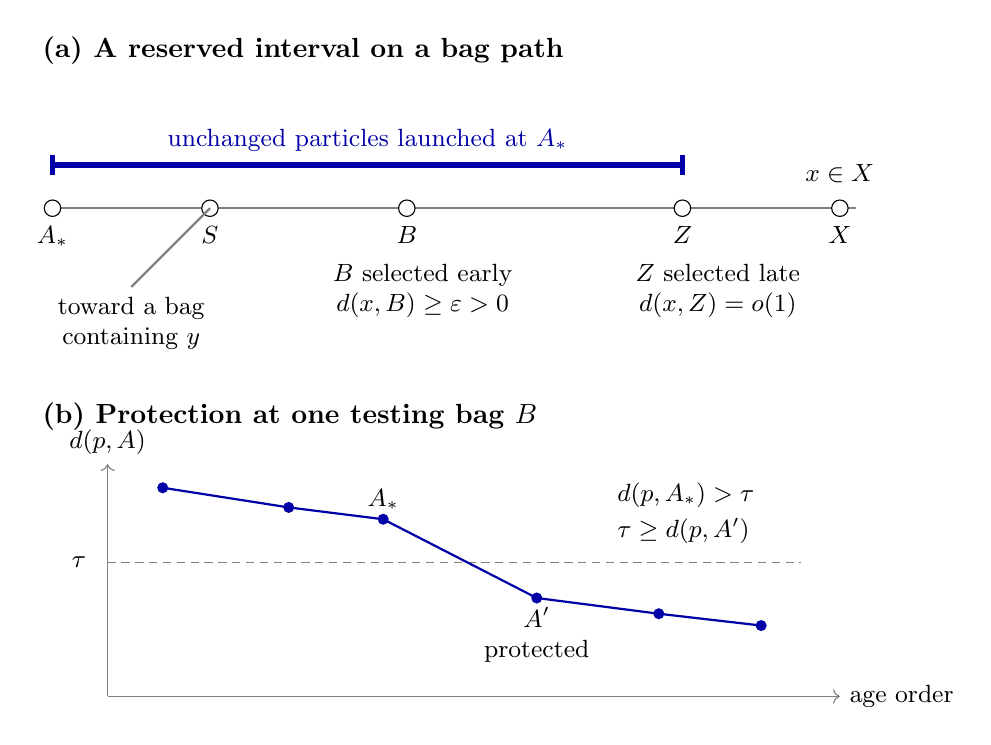
\begin{tikzpicture}[x=1cm,y=1cm,font=\small,
 bag/.style={circle,draw,fill=white,inner sep=2.1pt},
 retained/.style={blue!65!black,line width=2pt}]
 \node[anchor=west,font=\bfseries] at (-.25,2.0) {(a) A reserved interval on a bag path};
 \draw[gray,thick] (0,0)--(10.2,0);
 \foreach \x/\name in {0/A_*,2/S,4.5/B,8/Z,10/X} {
   \node[bag,label=below:$\name$] at (\x,0) {};
 }
 \draw[gray,thick] (2,0)--(1,-1);
 \node[below,align=center] at (1,-1) {toward a bag\\containing $y$};
 \draw[retained] (0,.55)--(8,.55);
 \draw[retained] (0,.42)--(0,.68);
 \draw[retained] (8,.42)--(8,.68);
 \node[blue!65!black,above] at (4,.6) {unchanged particles launched at $A_*$};
 \node[above,align=center] at (4.5,0) {\strut};
 \node[align=center] at (4.7,-1.05) {$B$ selected early\\$d(x,B)\ge\varepsilon>0$};
 \node[align=center] at (8.45,-1.05) {$Z$ selected late\\$d(x,Z)=o(1)$};
 \node[above] at (10,.2) {$x\in X$};
 \node[anchor=west,font=\bfseries] at (-.25,-2.65) {(b) Protection at one testing bag $B$};
 \draw[->,gray] (.7,-6.2)--(10,-6.2) node[right,black] {age order};
 \draw[->,gray] (.7,-6.2)--(.7,-3.25) node[above,black] {$d(p,A)$};
 \draw[gray,densely dashed] (.7,-4.5)--(9.5,-4.5);
 \node[anchor=east] at (.55,-4.5) {$\tau$};
 \draw[blue!65!black,thick] (1.4,-3.55)--(3,-3.8)--(4.2,-3.95)--(6.15,-4.95)--(7.7,-5.15)--(9,-5.3);
 \foreach \x/\y in {1.4/-3.55,3/-3.8,4.2/-3.95,6.15/-4.95,7.7/-5.15,9/-5.3}
  {\fill[blue!65!black] (\x,\y) circle (2pt);}
 \node[above] at (4.2,-3.95) {$A_*$};
 \node[below,align=center] at (6.15,-4.95) {$A'$\\protected};
 \node[anchor=west] at (7.05,-3.65) {$d(p,A_*)>\tau$};
 \node[anchor=west] at (7.05,-4.1) {$\tau\ge d(p,A')$};
\end{tikzpicture}
\caption{The two orders in the anchor argument.
In (a), the selected early bag $B$ and late terminal bag $Z$ lie in the
reservation of $A_*$; the branch toward $y$ makes $B$ a testing bag on
the path to $Z$. The horizontal axis records bag order, not metric
distance, and no first late or last early bag is depicted.
In (b), the entries are ordered by launch time in the list at $B$.
The distance list is nonincreasing. The immediate successor $A'$ is
protected when one of the thresholds $\tau=L/100$ or $\tau=JL$ lies
between its distance and that of $A_*$, where $L=d(p,q)$ is supplied
by Lemma~\ref{lem:anchor-obstruction}. All spacings are schematic.}
\label{fig:anchor-reservations}
\end{figure}


\begin{lemma}[Protection of the immediate successor]
\label{lem:protected-successor}
At any selected early eviction test $B$, suppose the immediate successor
$A'$ of $A_*$ in the inclusive cache list was launched at or after $S$.
Then $A'$ is protected and cannot be evicted at this test.
\end{lemma}

\begin{proof}
Let $p\in B$ be nearest to $x$, and put $\delta=d(x,B)$.
If $A'$ is the current proposal, $d(p,A')=0$.  Otherwise its reservation
lasts from its launch through $B$, and its launch lies on the bag path
from $y$ to $B$.  Equation~\eqref{eq:anchor-launch-test} yields
\[
 b_kd(p,A')\leq D(y,p)\leq D(y,x)+U\delta.
\]
Because $\delta$ is early, $D(y,x)/\delta$ is infinitesimal.  The choice
of $K$ in \eqref{eq:anchor-parameters} consequently gives, eventually,
\begin{equation}\label{eq:successor-distance-bounds}
 d(p,A')\leq K\delta.
\end{equation}
This inequality also holds for a proposal.  Monotonicity of distances
along the path gives $d(x,A')\leq d(x,S)=1$, so in all cases
\begin{equation}\label{eq:successor-absolute-bounds}
 d(p,A')\leq\delta+1\leq2,
 \qquad d(p,A_*)\geq D_0-\delta\geq D_0-1.
\end{equation}

Choose $q$ from Lemma~\ref{lem:anchor-obstruction} and write $L=d(p,q)$.
There are two alternatives.  If $L\leq300$, then
\[
 JL\geq\frac{J\delta}{4}>K\delta\geq d(p,A'),
 \qquad JL\leq300J<H-1<D_0-1\leq d(p,A_*).
\]
If $L>300$, then
\[
 \frac{L}{100}>3>2\geq d(p,A'),
 \qquad \frac{L}{100}\leq\frac{D_0}{10}
       <D_0-1\leq d(p,A_*).
\]
In either case one of the thresholds in \eqref{eq:cache-thresholds}
lies strictly below $d(p,A_*)$ and at or above $d(p,A')$.
Since the distance list is nonincreasing and $A'$ immediately follows
$A_*$, it is precisely the entry protected by this drop.
\end{proof}

\begin{lemma}[A younger crossing anchor exists]
\label{lem:younger-crossing}
Under the normalized failure assumption \eqref{eq:normalized-failure},
there is a crossing anchor younger than $A_*$.
\end{lemma}

\begin{proof}
Inspect the inclusive cache list at the insertion test at $S$.
By Lemma~\ref{lem:old-distant-anchor}, $A_*$ was launched strictly
above $S$, so this is indeed a non-root insertion.  Consider the
younger entries whose launches were strictly above $S$.  Their number
is bounded by $n_0+1$; by a finite ultrafilter alternative, enumerate
them as a fixed finite list of anchor sequences.
These are all the anchors younger than $A_*$ and launched above $S$
that can be present at any later test: an evicted reservation never
returns, and every later launch is at or below $S$.

Each has effective start $S$, which is early.  If any had a late terminal
bag, it would be a crossing anchor younger than $A_*$.  By the choice
of $A_*$, every one must instead have an early terminal bag.  Such a bag
is its actual eviction bag, since the endpoint $X$ is late.

If this finite list is nonempty, take the latest of these eviction
times, say $B_0$.  It is early.  At this test an old younger anchor is
actually evicted, so the new proposal is retained: exactly one entry
is evicted at an insertion.  The anchor $A_*$ remains present, because
its terminal time is late.  Immediately after this eviction no younger
anchor launched above $S$ remains, and the retained proposal ensures
that at least one younger entry exists.  Therefore $A_*$ has an
immediate successor $A'$ whose launch is at or after $S$.

If the finite list is empty, the proposal at $S$ is itself the immediate
successor of $A_*$.  It is retained automatically when there is space;
at a full insertion Lemma~\ref{lem:protected-successor} prohibits its
eviction.  Thus in this case too there is an immediate successor $A'$
launched at or after $S$, present just after an early test $B_0=S$.

Fix this successor $A'$.  Its launch is no later than the early time
$B_0$, so its effective start is early.  If its terminal bag is late,
it is the required younger crossing anchor.  Otherwise its terminal
bag is an early eviction time $B_1$.  The anchor $A_*$ is still present
at $B_1$.  While both anchors remain, $A'$ remains the immediate
successor: there was no entry between them at $B_0$, and all subsequent
insertions are younger than $A'$.  Hence
Lemma~\ref{lem:protected-successor} prohibits eviction of $A'$ at
$B_1$, a contradiction.

This argument selected only a bounded list of anchors, its last
eviction, and one successor's terminal time.  It does not use induction
over an unbounded or limiting order of early times.
\end{proof}

\begin{proof}[Proof of Proposition~\ref{prop:combined-lower}]
If no such constant existed, choosing ratios smaller than $1/i$ would
give \eqref{eq:failed-lower-comparison}.  The normalization above and
Lemmas~\ref{lem:youngest-crossing}--\ref{lem:younger-crossing} would then
produce a crossing anchor younger than the youngest crossing anchor.
This contradiction rules out a sequence of ratios tending to zero.
Their infimum over all nontrivial admissible examples and all distinct
pairs is therefore positive.  Choose $\lambda_k$ no larger than that
infimum.  Equal pairs and the one-vertex graph satisfy
\eqref{eq:combined-lower} automatically.
\end{proof}

\section{Completing the embedding}\label{sec:conclusion}

\begin{proof}[Proof of Theorem~\ref{thm:main}]
The one-vertex graph is immediate. For every other admissible graph,
Proposition~\ref{prop:cobag} and the anchor construction give finite cut
pseudometrics $D_{\mathrm{bag}}$ and $D_{\mathrm{anc}}$ satisfying the uniform upper
bounds established there. Proposition~\ref{prop:combined-lower} gives a
constant $\lambda_k>0$, depending only on $k$, such that their sum $D$ obeys
\[
 \lambda_k d(u,v)\le D(u,v)\le (U_{\mathrm{bag}}+U)d(u,v)
 \qquad(u,v\in V).
\]
For each construction, average the mass assigned to each labeled cut
$\omega\in\{0,1\}^V$.  The common total sweep mass is finite and
deterministic for the given graph, so all these expected masses are
finite.  Adding the two measures and identifying $\omega$ with
$A=\{v:\omega(v)=1\}$ gives
\[
 D(u,v)=\sum_{A\subseteq V}w_A
   |\mathbf{1}_A(u)-\mathbf{1}_A(v)|,
 \qquad w_A\ge0.
\]
The map
\[
 F(v)=\bigl(\lambda_k^{-1}w_A\mathbf{1}_A(v)\bigr)_{A\subseteq V}
       \in\ell_1^{\,2^{|V|}}(\mathbb R)
\]
therefore has distance $D/\lambda_k$ and satisfies
\eqref{eq:main-embedding} with
$C_k=(U_{\mathrm{bag}}+U)/\lambda_k$.
Every constant used to obtain this comparison depends only on $k$.
\end{proof}

The compactness argument establishes a positive uniform lower factor without
an explicit numerical estimate; the embedding assertion requires only its
existence.

\begin{thebibliography}{99}

\bibitem{AFGN22}
Ittai Abraham, Arnold Filtser, Anupam Gupta, and Ofer Neiman.
Metric embedding via shortest path decompositions.
\emph{SIAM Journal on Computing} \textbf{51}(2):290--314, 2022.
\href{https://doi.org/10.1137/19M1296021}{doi:10.1137/19M1296021}.

\bibitem{AR98}
Yonatan Aumann and Yuval Rabani.
An $O(\log k)$ approximate min-cut max-flow theorem and approximation algorithm.
\emph{SIAM Journal on Computing} \textbf{27}(1):291--301, 1998.
\href{https://doi.org/10.1137/S0097539794285983}{doi:10.1137/S0097539794285983}.

\bibitem{CJLV08}
Amit Chakrabarti, Alexander Jaffe, James R. Lee, and Justin Vincent.
Embeddings of topological graphs: Lossy invariants, linearization, and 2-sums.
In \emph{49th Annual IEEE Symposium on Foundations of Computer Science},
pp.~761--770. IEEE, 2008.
\href{https://doi.org/10.1109/FOCS.2008.79}{doi:10.1109/FOCS.2008.79}.

\bibitem{ChalermsookEtAl}
Parinya Chalermsook, Matthias Kaul, Matthias Mnich, Joachim Spoerhase,
Sumedha Uniyal, and Daniel Vaz.
Approximating sparsest cut in low-treewidth graphs via combinatorial diameter.
\emph{ACM Transactions on Algorithms} \textbf{20}(1), Article~6,
pp.~1--20, 2024.
\href{https://doi.org/10.1145/3632623}{doi:10.1145/3632623}.

\bibitem{CGNRS06}
Chandra Chekuri, Anupam Gupta, Ilan Newman, Yuri Rabinovich, and Alistair Sinclair.
Embedding $k$-outerplanar graphs into $\ell_1$.
\emph{SIAM Journal on Discrete Mathematics} \textbf{20}(1):119--136, 2006.
\href{https://doi.org/10.1137/S0895480102417379}{doi:10.1137/S0895480102417379}.

\bibitem{CKR}
Eden Chlamt{\'a}{\v c}, Robert Krauthgamer, and Prasad Raghavendra.
Approximating sparsest cut in graphs of bounded treewidth.
In \emph{APPROX/RANDOM 2010}, Lecture Notes in Computer Science,
vol.~6302, pp.~124--137. Springer, 2010.
\href{https://doi.org/10.1007/978-3-642-15369-3_10}{doi:10.1007/978-3-642-15369-3\_10}.
Full version: \href{https://arxiv.org/abs/1006.3970v2}{arXiv:1006.3970v2}.

\bibitem{CohenAddadMomkeVerdugo}
Vincent Cohen-Addad, Tobias M{\"o}mke, and Victor Verdugo.
A 2-approximation for the bounded treewidth sparsest cut problem in FPT time.
\emph{Mathematical Programming} \textbf{206}:479--495, 2024.
\href{https://doi.org/10.1007/s10107-023-02044-1}{doi:10.1007/s10107-023-02044-1}.

\bibitem{ConroyFiltser25}
Jonathan Conroy and Arnold Filtser.
How to protect yourself from threatening skeletons:
Optimal padded decompositions for minor-free graphs.
In \emph{57th Annual ACM Symposium on Theory of Computing},
pp.~2281--2292. ACM, 2025.
\href{https://doi.org/10.1145/3717823.3718252}{doi:10.1145/3717823.3718252}.

\bibitem{FiltserEtAl}
Arnold Filtser, Tobias Friedrich, Davis Issac, Nikhil Kumar, Hung Le,
Nadym Mallek, and Ziena Zeif.
Optimal padded decomposition for bounded treewidth graphs.
\emph{TheoretiCS} \textbf{4}, Article~22, pp.~1--39, 2025.
\href{https://doi.org/10.46298/theoretics.25.22}{doi:10.46298/theoretics.25.22}.

\bibitem{GNRS}
Anupam Gupta, Ilan Newman, Yuri Rabinovich, and Alistair Sinclair.
Cuts, trees and $\ell_1$-embeddings of graphs.
\emph{Combinatorica} \textbf{24}(2):233--269, 2004.
\href{https://doi.org/10.1007/s00493-004-0015-x}{doi:10.1007/s00493-004-0015-x}.
\href{https://cs.nyu.edu/~ag10120/papers/focs99.pdf}{Author manuscript}.

\bibitem{GuptaTalwarWitmer}
Anupam Gupta, Kunal Talwar, and David Witmer.
Sparsest cut on bounded treewidth graphs: Algorithms and hardness results.
In \emph{45th Annual ACM Symposium on Theory of Computing},
pp.~281--290. ACM, 2013.
\href{https://doi.org/10.1145/2488608.2488644}{doi:10.1145/2488608.2488644}.
Full version: \href{https://arxiv.org/abs/1305.1347}{arXiv:1305.1347}.

\bibitem{LP13}
James R. Lee and Daniel E. Poore.
On the 2-sum embedding conjecture.
In \emph{29th Annual Symposium on Computational Geometry},
pp.~197--206. ACM, 2013.
\href{https://doi.org/10.1145/2462356.2492436}{doi:10.1145/2462356.2492436}.

\bibitem{LR10}
James R. Lee and Prasad Raghavendra.
Coarse differentiation and multi-flows in planar graphs.
\emph{Discrete \& Computational Geometry} \textbf{43}(2):346--362, 2010.
\href{https://doi.org/10.1007/s00454-009-9172-4}{doi:10.1007/s00454-009-9172-4}.

\bibitem{LS09Geometry}
James R. Lee and Anastasios Sidiropoulos.
On the geometry of graphs with a forbidden minor.
In \emph{41st Annual ACM Symposium on Theory of Computing},
pp.~245--254. ACM, 2009.
\href{https://doi.org/10.1145/1536414.1536450}
{doi:10.1145/1536414.1536450}.

\bibitem{LeeSidiropoulos}
James R. Lee and Anastasios Sidiropoulos.
Pathwidth, trees, and random embeddings.
\emph{Combinatorica} \textbf{33}(3):349--374, 2013.
\href{https://doi.org/10.1007/s00493-013-2685-8}{doi:10.1007/s00493-013-2685-8}.

\bibitem{LLR95}
Nathan Linial, Eran London, and Yuri Rabinovich.
The geometry of graphs and some of its algorithmic applications.
\emph{Combinatorica} \textbf{15}(2):215--245, 1995.
\href{https://doi.org/10.1007/BF01200757}{doi:10.1007/BF01200757}.

\bibitem{OpenAIPlanar}
OpenAI.
Planar Graph Metrics Embed into $L_1$ with Constant Distortion.
OpenAI Math Release preprint
\href{https://github.com/openai/math/blob/main/preprints/Planar-Graph-Metrics-Embed-into-L1-with-Constant-Distortion-September-23-2026/paper.pdf}{OAI:Planar-Graph-Metrics-Embed-into-L1-with-Constant-Distortion-September-23-2026},
2026.

\bibitem{RS86Planar}
Neil Robertson and P. D. Seymour.
Graph minors. V. Excluding a planar graph.
\emph{Journal of Combinatorial Theory, Series B}
\textbf{41}(1):92--114, 1986.
\href{https://doi.org/10.1016/0095-8956(86)90030-4}
{doi:10.1016/0095-8956(86)90030-4}.

\end{thebibliography}

\end{document}
